\documentclass[en]{pracamgr}

\usepackage{float}
\usepackage{xpatch}
\usepackage{listings}
\usepackage{minted}
\usepackage{tikz-cd}
\usepackage{amsmath}
\usepackage{amssymb}
\usepackage{hyperref}
\usepackage{epigraph}
\usepackage{amsfonts}
\usepackage{ragged2e}
\usepackage{graphicx}
\usepackage{adjustbox}
\usepackage{breakcites}


\definecolor{string_color}{rgb}{0.12, 0.3, 0.17}
\lstdefinestyle{basic}{
  basicstyle=\ttfamily,
  numbers=left,
  numberstyle=\color{gray}\ttfamily,
  numbersep=5pt,
  backgroundcolor=\color{white},
  showspaces=false,
  showstringspaces=false,
  showtabs=false,
  rulecolor=\color{black},
  captionpos=b,
  commentstyle=\color{gray},
  stringstyle=\color{green},
  keywordstyle=\bfseries\rmfamily,
  emphstyle={\bf},
  commentstyle=\it,
  stringstyle=\ttfamily\color{string_color},
  xleftmargin=2pt,
  stepnumber=1,
  numbersep=5pt,
  belowcaptionskip=\bigskipamount,
  belowskip=\bigskipamount,
  aboveskip=\bigskipamount,
  captionpos=b,
  % escapeinside={*'}{'*},
  tabsize=2,
  columns=flexible,
  keepspaces=true
}


\lstdefinelanguage{pseudocode}
{
  morekeywords={let, for, in, constraint, zip, fold_left, length, do, int, reachable, unreachable,
    if, then, else, fun, end, return, var, filter, while, true, false, error, not},
  morecomment=[l]{--},
  morestring=[b]",
  mathescape,
  style=basic,
}

\lstdefinelanguage{smtlib}
{
  morekeywords={assert, push, pop, check, sat, sat, unsat, declare, const, Int, Bool},
  morecomment=[l]{;},
  morestring=[b]",
  style=basic,
  keywordstyle=\bfseries\ttfamily,
}

\lstdefinelanguage{bnf}
{
  morekeywords={::=},
  morecomment=[l]{//},
  morestring=[b]',
  style=basic,
}

\lstdefinelanguage{sophia}
{
  language=caml,
  keywords={contract, include, let, switch, type, record, datatype, if, elif, else, function,
    stateful, payable, true, false, mod, public, entrypoint, private, indexed, namespace,
    interface, main, int, bool, list, address, require},
  sensitive=true,
  morecomment=[l]{//},
  morestring=[b]",
  style=basic,
}

\lstdefinelanguage{erl}
{
  morekeywords={length, lists, length, zip, zip3, spec},
  sensitive=false,
  morecomment=[l]{\%},
  morestring=[b]",
  style=basic,
  literate=
  {->}{$\to{}$}{1}
}


\graphicspath{ {./images/} }

\newenvironment{code}[4][htp]
{\VerbatimEnvironment
  \begin{figure}[#1]
    \centering
    \ifthenelse{\equal{#3}{}}{}{\caption{#3}}
    \ifthenelse{\equal{#3}{}}{}{\label{#4}}
\begin{minted}[linenos]{#2}}
    {\end{minted}\end{figure}}

\usemintedstyle{autumn}

\xapptocmd{\ttfamily}{\frenchspacing}{}{}


\autor{Radosław Jan Rowicki}{386088}

\title{Liquid types for verification of smart contracts}
\titlepl{Weryfikacja inteligentnych kontraktów przy pomocy logicznie
  kwalifikowanych typów danych}
\kierunek{Computer Science}

\opiekun{PhD. Ulf Norell\\
  University of Gothenburg\\
}
\opiekunuw{PhD. Marcin Benke\\
  University of Warsaw\\
}

\date{September 2021}

%Podać dziedzinę wg klasyfikacji Socrates-Erasmus:
\dziedzina{
  11.3 Informatics
}

\klasyfikacja{
  D Software\\
  D.1 Programming Techniques\\
  D.1.1 Functional Programming\\
  D.3 Programming Languages\\
  D.3.3 Language Constructs and Features\\
  F Theory of Computation\\
  F.3 Logics and Meanings of Programs\\
  F.3.2 Specifying and Verifying and Reasoning about Programs }

\keywords{liquid types, smart contracts, formal verification, dependent types,
  functional programming, blockchain}

\newtheorem{defi}{Definition}[section]

\AtBeginDocument{%
  \providecommand\BibTeX{{%
    \normalfont B\kern-0.5em{\scshape i\kern-0.25em b}\kern-0.8em\TeX}}}

\begin{document}

\maketitle

\center \subsection*{Acknowledgements}

\justify First of all, I would like to thank my supervisor, Ulf Norell, for
supporting me during my work by inspiring me with ideas, giving numerous
valuable comments, and discussing various solutions. I am also grateful for our
cooperation in developing the compiler of Sophia, during which I learned a lot
about implementing programming languages. Next, I appreciate the support from
Marcin Benke representing the University of Warsaw, who coordinated the formal
side of my thesis. Furthermore, I am thankful for what he taught me about type
systems and semantics of functional languages.

\justify This work has been a subject of the 0135 grant of the Aeternity Crypto
Foundation ``Logic Qualified Data Types for Sophia''. I hereby thank Lydia
Atanassova representing the Foundation for her assistance regarding the grant
application. I would also like to thank all my colleagues from the {\ae}ternity
Core--Dev team for being exceptionally inspiring professionals, with whom it was
a big pleasure to work.

\justify Last but not least, I would like to thank my girlfriend, Karolina
Tudelska, for her moral support and for providing me with priceless advice on
writing texts in English.

\begin{abstract}
  In recent years smart contracts have been developed within the blockchain
  technology as a trustless tool for managing digital assets, many of which are
  of considerable value. Due to the nature of blockchains, smart contracts are
  vulnerable to bugs, because once deployed, they cannot be fixed. This can have
  wide-ranging financial consequences, as cryptocurrencies and NFTs rapidly gain
  popularity. Therefore, a great need for meticulous audits emerges, so the
  vulnerabilities can be found and mitigated before they cause harm.

  This work presents liquid types as a method of computer-aided verification of
  smart contracts. The analysed implementation named Hagia is an extension of
  the type system of the Sophia language, which has been designed for smart
  contract development on the {\ae}ternity blockchain. Liquid types have already
  found application in many projects written in functional languages such as
  OCaml or Haskell. The presented algorithms and discussions provide a framework
  for understanding the key concepts of the liquid inference, use cases and the
  benefits of the proposed solution in the context of smart contract
  development.
\end{abstract}

\chapter*{Changelog}

This is a revisited version that was not the subject of the defence, nor the
changes listed here have been reviewed by the supervisors. The modifications
are mostly cosmetic and should not change meanings of sentences.

\subsection*{Version 1.0.1}

\begin{itemize}
\item Added this changelog.
\item Fixed typo in "Implementation" chapter: occuring -> occurring.
\item Added and removed a few commas in "Implementation" chapter. 
\item Fixed typos in the algorithm for splitting subtyping of functions
  (sub -> sup in some places).
\end{itemize}

\tableofcontents

\chapter{Introduction}

\section{Context}

In the last two decades, the blockchain technology \cite{Nakamoto:2008:RBP} has
emerged as a revolutionary approach to business \cite{noyen2014money,
  petukhina2020investing}, web services \cite{terzi2019blockchain} and
documentation of certain events, such as ownership transfers
\cite{wang2021nonfungible}. Many famous features and use cases of modern
blockchains highly rely on smart contracts \cite{khan2021}, first introduced at
2013 as one of the main features of Ethereum \cite{wood2014ethereum}. Smart
contracts allow performing a variety of actions related to cryptocurrencies in a
zero-trust manner making them a widely practised way of making anonymous
agreements, trading, and more.

The invention of smart contracts gave birth to a new programming paradigm. As
explained in the upcoming sections, decentralised applications have very
specific priorities regarding their implementations and take into consideration
issues that are usually not present in classical computer programs. One of their
most prominent value is having very defensive code, first aim of which is to
reduce the number of errors and unexpected behaviours as soon as it is possible.
While it is important to virtually all programs, smart contracts rely on it
exceptionally strongly, because they are impossible to be fixed after deployment
and the causalities of bugs in them can be frighteningly expensive.

In this document we present Hagia --- a liquid type refinement system that
supports verification of smart contracts written in the Sophia language
\cite{sophia}. Hagia has been written as an extension to the Sophia compiler and
its code is available on GitHub\footnote{Please refer to the related pull
  request at https://github.com/aeternity/aesophia/pull/334. The whole source
  code of the upgraded compiler can be previewed in the forked \texttt{aesophia}
  repository at https://github.com/radrow/aesophia/tree/hagia.}. This
dissertation focuses on its implementation and application for the smart
contract development, along with the theory behind it.

The following sections familiarise the reader with the idea of blockchain and
smart contracts --- first in a more popular context of the Ethereum network and
then moving to the case study of this work, which is the {\ae}ternity
blockchain. The next chapters introduce the Sophia language, discuss the need
for advanced type systems and present liquid types as a solution for the most
common issues of smart contracts. The \autoref{implementation} explains the main
algorithms and logics of Hagia and presents the source code of the most
important functions. The detailed implementations can be found in the linked
GitHub repository. At the end there is a presentation and discussion on how
Hagia enhances Sophia and what is its value for the ecosystem of {\ae}ternity.

\section{Blockchain}

Blockchain is a distributed data structure resembling a singly-linked list. The
main unit of a blockchain is a \emph{block}. Each block consists of a collection
of events called \emph{transactions} which most often represent virtual token
transfers and interactions with smart contracts. To keep the integrity of the
whole structure, every block stores the hash of the previous one making it
always clear which chain it belongs to and what its position is. Because of this
connection, changing, adding or removing any block in the middle requires
updating all following blocks as well, making forging chains virtually
impossible.

The participants of the network are usually called \emph{peers}, and those who
produce blocks are referred as \emph{miners}. Since miners are responsible for
keeping the blockchain alive, they are compensated for their work by being
credited with rewards in tokens and transaction fees of other peers. These fees
make denial-of-service attacks expensive and incentivise miners to validate
transactions and register them on the chain.

\begin{figure}[h]
  \caption{Blockchain visualisation}
  \centering
  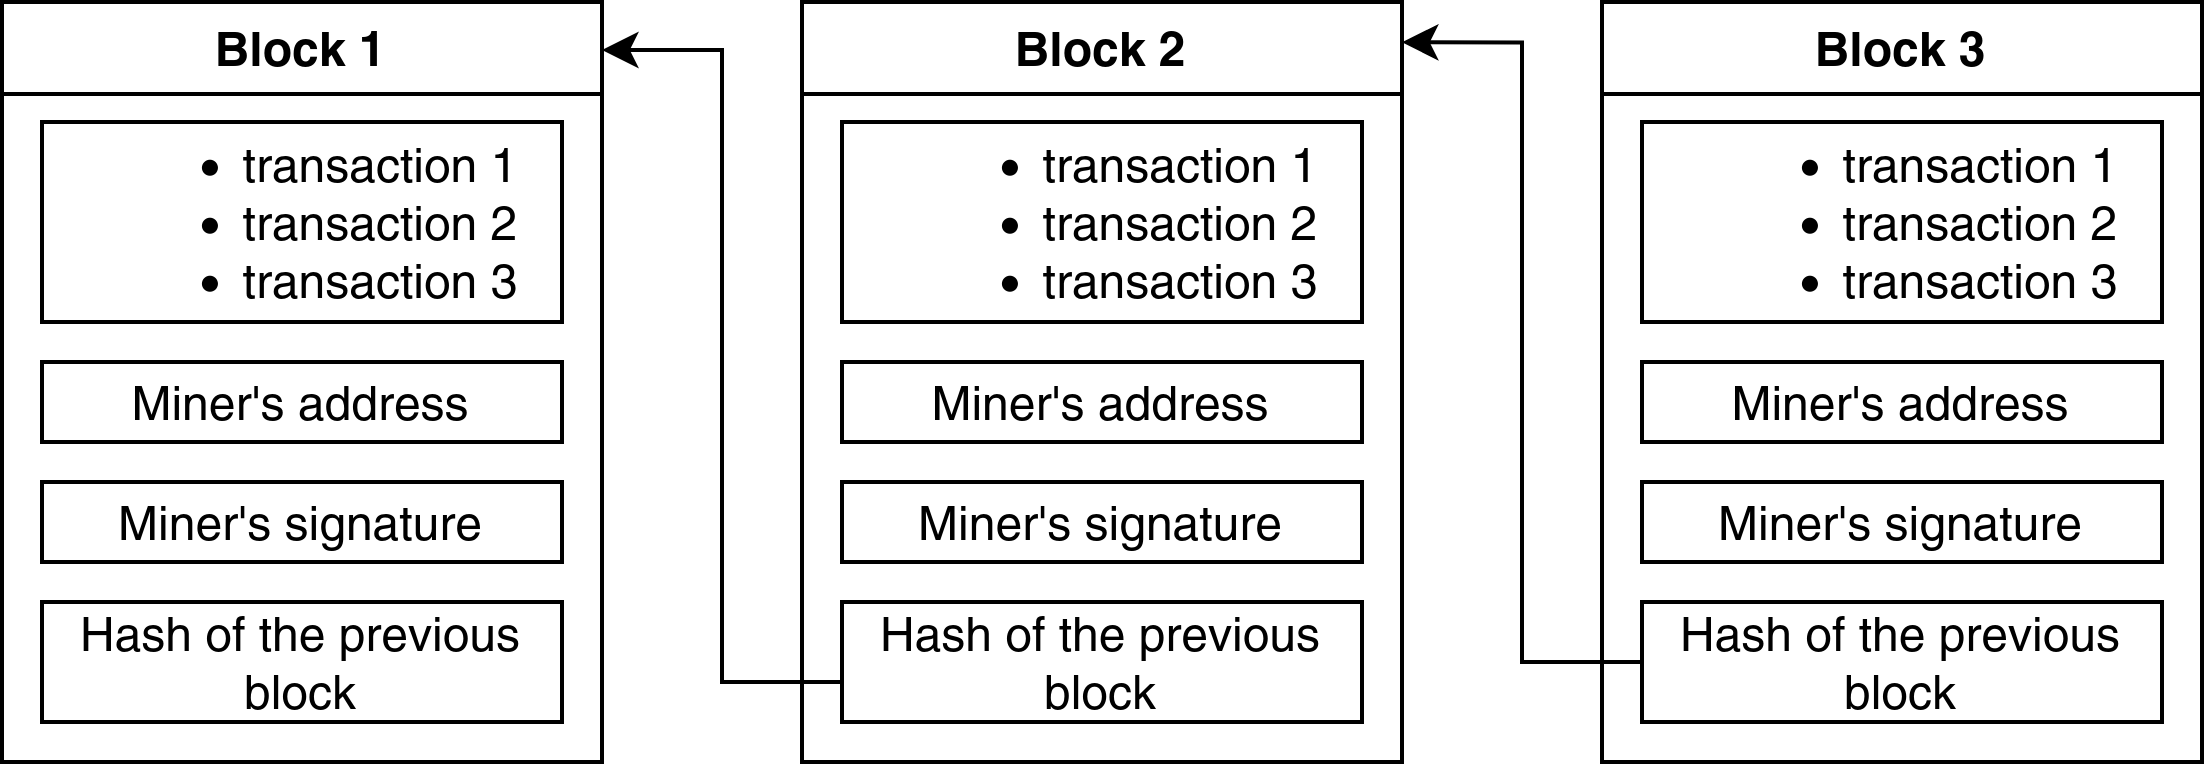
\includegraphics[scale=1]{blockchain}
\end{figure}

Each peer in the network is expected to keep at least some suffix of the chain,
so they do not need to rely on any centralised entity. Lack of a single point of
truth makes malicious peers, data races and hardware limitations a danger for
the integrity of the whole system, thus several algorithms to solve the problem
of synchronisation have been invented. The most popular ones are Proof of Work
(PoW) \cite{Nakamoto:2008:BPP} and Proof of Stake (PoS) \cite{King:2012:PPP}.
The former gains the security by forcing the peers to solve computationally hard
tasks, while the latter hands the right of producing new blocks to randomly
chosen peers based on the number of tokens they possess.

Such design aims to make the events on the chain immutable as soon as it is
possible. Owing to this, once a transaction has been placed on a blockchain, it
is nearly impossible to roll it back, because it would require convincing most
of the participants that the change is justified and shall not break any
assumptions. Consequently, no authority is able to undo an unwanted or misguided
action, assuming the network is properly secured.

\section{Smart contracts}

A smart contract is a computer program that acts as a first-class citizen in the
network. It owns tokens, may interact with other contracts, perform spend
transactions and accept incoming transfers. Due to the fact it lives entirely on
a blockchain, its behaviour is strictly defined by its immutable source code.

The most prominent smart contract language is Solidity, which compiles to the
Ethereum Virtual Machine (EVM). It is an imperative language highly influenced
by C and JavaScript, which supports some object-oriented programming features.
The EVM is a classical stack machine which additionally provides operations for
blockchain interaction.

Smart contracts allow making actual agreements between parties. As soon as all
the participants reach a consensus that the source code of a contract describes
the rules they want to follow, they can deploy it onto the chain and interact
with it. From this point on, the contract shall respond to their queries, manage
tokens and provide access to certain actions realising its purpose independently
and securely.

A basic example of such agreement would be a crowdfunding initiative: the
contract could accept and register incoming transfers and once the required
amount is reached, pay it out to the beneficiary. If the contract fails to
gather a certain amount up to a defined point in time\footnote{Time in the
  context of blockchains is usually measured in blocks which, in contrary to
  seconds, is not prone to synchronisation issues.}, it pays the tokens back to
the supporters. The investors do not need to worry if the rules are going to be
respected, as the power of the network secures it firmly.

One of the concerns arising from allowing computationally universal algorithms
to be executed on the chain is that not every peer might be able to evaluate
them entirely due to resource limitations. While there are some attempts to
statically put restrictions on the time and memory consumption, in general case
it is even impossible to tell if a given program ever returns \cite{turing1937}.
Owing to this, some additional mechanisms have to be introduced to eliminate the
risk of forcing peers to perform unrealistic computations.

One of the solutions involves so-called \emph{gas} as a remedy to that
problem \cite{wood2014ethereum}. Gas is a resource that must be acquired by the
caller before the contract is invoked. Each operation of the virtual machine
incurs a non-refundable gas cost. When the gas declared by the caller is
exhausted, execution stops and the transaction is reverted. The price of it and
the costs of particular instructions are adjusted so casual actions are
affordable, but performing heavier computations is costly.

The immutability of transactions gives a raise to a more problematic issue: if a
bug is spotted once the contract has been deployed, it cannot be fixed. The only
way to get rid of it is to create a new contract, migrate the state from the old
one and make all the parties aware of the issue\footnote{Of course, one must
  keep in mind that they do not have to agree on that and nothing stops them
  from abusing the contract.}. So far errors in smart contracts have made
significant harm to many entities exposing them to very damaging
loses \cite{peterjoost2018, olha.hlebiv2018, bishwascgupta2019, mattsuiche2017,
  christianreitwiessner2016}. Because of it, there is a great need for testing
and verifying contracts before they are let to the network.

\section{{\ae}ternity}

The case study of this research is the {\ae}ternity blockchain \cite{aeternity}.
At the time of writing it is a PoW chain implementing the BitcoinNG
\cite{Gencer:2017:SBT} protocol\footnote{As of September 2021 there are works on
  a custom protocol called hyperchains \cite{hyperchains}, which was first
  presented on 25th of August 2020}. It is highly inspired by Ethereum and
implements smart contracts, a naming system \cite{aens,
  brantlymillegannickjohnson2021}, oracles \cite{oracles} and state channels
\cite{state_channels, state_channels_eth}. One of the things that distinguish
{\ae}ternity from other chains is a custom smart contract programming language,
Sophia, which compiles to a proprietary virtual machine called Fast Aeternity
Transaction Engine (FATE) \cite{fate}. It shall be the main subject of analysis
in this work.

The project was established in 2017 by Yanislav Malahov and funded in an
ICO crowdfunding \cite{crunchbase2017}. The core code is written in Erlang with
some key parts implemented also in Elixir and Rust. It is entirely open source
and can be inspected in the official GitHub repository:
\url{https://github.com/aeternity}.

\chapter{The Sophia language}
\label{chapter_sophia}

\section{Language overview}

Sophia is a domain-specific language that targets smart contracts on the
{\ae}ternity blockchain. It belongs to the ML family being a statically and
strongly typed functional language supporting parametric polymorphism with fully
developed type inference. It was created in 2017 by Ulf Norell, Hans Svensson,
Erik Stenman and Tobias Lindahl as a part of the {\ae}ternity core node, and was
later separated as a stand-alone tool equipped with a command line interface, an
HTTP service and an interactive REPL. For a first look at the syntax, an example
of a Sophia contract that serves as a factorial calculator is presented in
\autoref{example_factorial}.

\begin{code}[!hbt]{lexers/sophia.py:SophiaLexer -x}{Factorial contract}{example_factorial}
contract Fac =
  entrypoint
    factorial : int => int
    factorial(n) =
      if(n == 0) 1
      elif(n > 0) n * factorial(n - 1)
      else 0
\end{code}

One of the key reasons for making it functional is the belief that this paradigm
provides decent security against common bugs \cite{Hughes89whyfunctional}. The
strict type system catches many domain-related errors and referential
transparency\footnote{Technically speaking, Sophia is not entirely referential
  transparent due to some impure constructions which shall be discussed later
  on.} simplifies reasoning about blocks of code, allowing the reader to analyse
it without having to mind the context of the global variables. Moreover, the
reactive style of programming weaves in the transaction-driven nature of
blockchains exceptionally well.

The language is designed for the blockchain interaction. Among others, it
provides instructions for checking the number of tokens transferred with the
current call, the entity that performed or originated\footnote{The difference
  between these two emerges when a contract is calling another contract. The
  \emph{caller} is the direct entity that initiated the call, while the
  \emph{origin} is the peer who published the call transaction.} the call,
balance of any address (including own) and performing spend transactions. There
is also a rich library of cryptographic functions, data structure algorithms and
functional combinators \cite{sophia_stdlib}.

Despite being a declarative language, Sophia does offer a limited control over a
mutable state. The programmer is allowed to define a special type \texttt{state}
and is given a control over a single variable of it which can be freely modified
across the execution. There is a dedicated entrypoint \texttt{init} which is
called only once during the contract initialisation and sets up the initial
state. The state persists between calls and is the main way of storing
information on the chain by smart contracts.

Sophia divides functions by three categories: statefulness, payability and
exposure to the outer world:

\begin{itemize}
\item For a function to be allowed to directly or indirectly modify state of the
  contract\footnote{That includes not only the \texttt{state} variable, but also
    the balance.}, it must be declared with the \texttt{stateful} keyword. This
  restriction effectively brings back the benefits of immutability and purity.
  Non-stateful functions can read the state freely, though.
\item A function that is \texttt{payable} is allowed to be called along with a
  token transfer to the contract. Making it explicit can prevent accidental
  spends by calling an entrypoint that is not prepared to handle the income
  properly.
\item As for exposure, functions that are supposed to be called from the outside
  (that is, by users or other contracts) have to be declared as
  \texttt{entrypoint}s instead of \texttt{function}s. This requirement allows
  keeping internal algorithms safe from unwanted calls, which could be dangerous
  considering the fact that they might operate on some intermediate state with a
  malformed structure.
\end{itemize}

For an example of a stateful contract please refer to the
\autoref{example_factorial_stateful} which presents a factorial calculator that
additionally counts and stores the number of its uses.

\begin{code}[htb]{lexers/sophia.py:SophiaLexer -x}{Counting factorial contract}{example_factorial_stateful}
contract Fac =
  type state = int
  entrypoint init() = 0

  stateful entrypoint fac(n) =
    require(n >= 0, "INVALID_ARG")
    put(state + 1)
    fac_internal(n, 1)

  function fac_internal(n, acc) =
    if(n == 0) acc
    else fac(n - 1, acc * n)

  entrypoint get_uses() = state
\end{code}

This document describes the 5.0.0 version of Sophia. However, at the time of
writing 6.0.2 is released featuring introspection of other contracts' byte code
and dynamic creation of new contracts. Although the presented type refinement
system does work well with the recent version, the new functionalities are not
taken into account.

\section{Syntax}

The structure of a Sophia program is split into three layers:

\subsubsection{Top level}

This is the root of a Sophia file. It contains directives for the compiler,
\texttt{include} statements, namespaces, contract interfaces and the main
contract definition. The last one is the actual body of the entity to be
deployed onto the blockchain. Namespaces aid the hermetisation and help keeping
tidy structure by dividing logic into separate modules. Contract interfaces
contain only entrypoint signatures and possibly type definitions which are
required for the cross-contract interaction. A valid Sophia program requires
exactly one contract definition and any number of contract declarations and
namespaces above it. At this level, the entities are processed top-down making
mutual recursion impossible.

The syntax of the top level can be visualised as presented in the
\autoref{top_level_syntax_example} (please refer to the
\autoref{full_sophia_syntax} for the full BNF grammar).

\begin{code}[H]{lexers/sophia.py:SophiaLexer -x}{Top level syntax example}{top_level_syntax_example}
// Compiler version pragmas
@compiler >= 5.0.0
@compiler < 6.0.0

// External file loading
include "List.aes"

// Namespace
namespace Lib =
  /* [Contract level] */

// Contract definition
contract Main =
  /* [Contract level] */
\end{code}


\subsubsection{Contract level}

This is the place where the definitions of functions and custom data types are
written. This time, the entities are processed in a way that allows mutual
recursion for functions, but not for data types. In case of contracts, functions
are divided into \texttt{entrypoint}s (public) and \texttt{function}s (private),
and for namespaces there are respectively \texttt{function}s and \texttt{private
  function}s. As stated before, each of these can be additionally equipped with
\texttt{payable} and \texttt{stateful} annotations.

Example syntax on this level is presented in the
\autoref{contract_level_syntax_example}.

\begin{code}[H]{lexers/sophia.py:SophiaLexer -x}{Contract level syntax
    example}{contract_level_syntax_example}
// Type alias
type i = int

// Record
record point = {x : i, y : i}

// Variant type (ADT)
datatype closed_int = NegInf | Int(i) | PosInf

// Single-clause function definition
function f(x) =
  /* [Function level] */

// Multi-clause function definition
function g : int => int  // Type declaration is optional
         g(0) = /* [Function level] */
         g(n) = /* [Function level] */

// Stateful function. Only in contracts.
stateful function h(x : int) : int * int = // Returns a tuple of two ints
  /* [Function level] */

// Stateful payable entrypoint. Only in contracts.
stateful payable entrypoint q() : unit = // Zero-tuple is referred as unit
  /* [Function level] */

// Private function. Only in namespaces.
private function w() : closed_int =
  /* [Function level] */

// Entrypoint declaration. Only in contract interfaces.
entrypoint e : (int, bool, string) => option(int * bool * string)
\end{code}

\subsubsection{Function level}

At the function level the actual algorithms are defined. The syntax is mostly
compatible with the Standard Meta-Language with some minor differences in the
blocks' layout, lambda definitions and imperative constructions. The most
notable change is the support for higher arity functions, which is normally
achieved with tuples or currying in other languages from the ML family.

\autoref{function_level_syntax_example} shows a selection of statements and
expressions that may appear here.

\begin{code}[H]{lexers/sophia.py:SophiaLexer -x}{Function level syntax
    example}{function_level_syntax_example}
require(state.size < 0, "STATE TOO LOW") // Data validation
let x = 10
let sqr(n) = n * n
if(state.size > x)
  abort("STATE TOO BIG") // Throwing an error
else
  let payload : list(int) = state.payload
  switch(payload)
    []   => 0
    h::t =>
      h * List.sum([a + 1 | a <- t]) // List comprehension
\end{code}


\autoref{example_contract_full} provides an example of a complete and compilable
contract presenting the most prominent features of the language. It shows a full
program structure, interaction with other contracts and some mock data
validation. Again, for the full reference please consult the appendix.

\begin{code}[!hb]{lexers/sophia.py:SophiaLexer -x}{A more complex Sophia contract example}{example_contract_full}
include "List.aes"

contract IntegerService =
  entrypoint retrieveInts : () => list(int)

namespace Validation =
  function validate(x : int) : bool =
    if(x >= 0)
      factorial(x) mod 2 == 0
    else false

  private function factorial(x) =
    switch(x)
      0 => 1
      _ => x * factorial(x - 1)

contract Main =
  type state = list(IntegerService)
  entrypoint init() = []

  stateful entrypoint register(service : IntegerService) : unit =
    require(List.all(Validation.validate, service.retrieveInts()),
            "INVALID_SERVICE")
    put(service::state)

  payable entrypoint get() =
    require(Call.value > 0, "FEE_REQUIRED")
    state
\end{code}

\section{Type system}

The type system of Sophia is a super-set of the Hindley--Milner's \cite{hindley,
  milner}. It offers first-rank parametric polymorphism, higher order functions
and full type inference. One of the limitations is that Sophia requires all
local variable definitions to be monomorphic and not recursive, meaning that in
some situations auxiliary functions must be extracted up to the contract level.

Sophia supports other contracts as first-class values, meaning that they can be
handled as ordinary data. For instance, in the \autoref{example_contract_full}
the main contract stores a list of references to other contracts that are
supposed to implement the \texttt{IntegerService} interface. Verification if
that is actually the case is an obligation of the user, since FATE does not type
check external contracts entirely, but only calls to their entrypoints.

The programmer is given an ability to describe custom data types in a manner
similar to other ML-like languages, like OCaml \cite{ocaml} or Elm
\cite{elm2013}. There are three alternatives for it:

\begin{enumerate}
\item Type alias --- created with the \texttt{type} keyword. It provides a
  different name for an existing type and can always be inlined without
  breaking the semantics.
\item Record --- created with the \texttt{record} keyword. This construction is
  also known as \emph{named tuple} or \emph{struct} in other programming
  languages. It is a data structure that consists of other data under named
  positions called \emph{fields}.
\item Variant --- created with the \texttt{datatype} keyword. Formally it is a
  non-generalised algebraic data type, and allows forming disjoint unions and
  products of other types using named constructors. It is heavily inspired by
  many modern programming languages like Haskell, OCaml and Rust.
\end{enumerate}

In contrary to the referred languages, Sophia does not support recursive type
definitions, making some constructions like trees inexpressible. However, there
is a built-in inductive \texttt{list} data type, which follows the common for
functional languages convention of being either an empty list \texttt{[]} or a
construction \texttt{head::tail} where \texttt{head} the first element and
\texttt{tail} is the list of the rest.

The lack of tree-like structures is partially mitigated by the built-in
\texttt{map} data type. Since trees are frequently used to implement data
collections, hash tables serve more often than not well enough for their use
case. The values are flexible to be of any types, while keys are limited not to
be other maps, functions and polymorphic variables.

The types can be parameterised with other types. This is very useful for
generalising various patterns and providing more meaningful names for some
complex domains. The parameters must not accept further parameters, making
higher-kinded types disallowed in Sophia.

\section{Potential issues}

Despite being very defensive and restrictive, Sophia is not capable of checking
several important varieties of assumptions. Among others, there is no way to
statically verify properties of values within the provided types, such as
integer boundaries. This can be a significant issue with contracts that manage
and store tokens. While one can be sure that a variable representing the balance
of some address is an integer, the compiler shall not guarantee that its value
is always non-negative. Overseeing such assumptions can expose contracts to
exploitation and in the worst case tokens theft.

Because of that, entrypoints require explicit validation of the incoming data.
The type checker does not have information about the expectations regarding it,
so it will not remind the user about the need of checking them. This becomes an
issue when domains are restricted with additional assumptions, what happens for
example in the standard library for rational numbers, which represents fractions
using only positive integers. The library does not check if the input data is
well-formed for performance reasons. Therefore, if the provided utilities are
used on unverified data coming from outside of the contract, they may latently
produce invalid results.

It is also worth noting that FATE type checks data during execution only to some
limited extent. For instance, while it is able to distinguish a list from an
integer, it will struggle telling a difference between variants if their
definitions are similar enough. Moreover, record types are non-existent in FATE
and are reduced to tuples by the compiler. Consequently, if data is compatible
on the byte code level, it may be coerced to a different Sophia type in an
unsafe way, leading to an unexpected interpretation of it in the other contract.

This also brings back the previously mentioned problem of data validation. For
example, let us consider a contract that utilises rational numbers and a variant
type of a structure similar to the respresentation of fractions. In such a case,
both types may be mistaken with each other without throwing a runtime error, but
evaluating invalid computation instead. It is visualised in the
\autoref{fate_messup}, where the \texttt{ChickenField} contract is called with
swapped arguments. The real implementation of \texttt{scale\_chicken} will thus
handle \texttt{InTheAir(-1, 0)} as a malformed fraction representing a negated
division $-1/0$. This operation \emph{will} succeed, but shall return a
senseless value. For example if \texttt{spawn\_chicken\_with} is called with
\texttt{distance} equal to 2, the result will be \texttt{InTheAir(0, 0)} instead
of the expected \texttt{InTheAir(-5, 0)}. Note that the bug is not only about
misuse of data, but also creation of malformed structures which silently
propagate across the runtime.

\begin{code}[hb]{lexers/sophia.py:SophiaLexer -x}{Example of a bug breaking data
    assumptions}{fate_messup}
/* file: ChickenField.aes                                                     */
/* Contract mixing rationals and similarly structured variants                */

// Standard library namespace for rational numbers
namespace Frac =
  // A fraction is represented by either zero positive/negative pair of
  // numerator and denominator
  datatype frac = Neg(int, int) | Zero | Pos(int, int)

  ...

contract ChickenField =
  // Datatype describing coordinates of a chicken in several states
  datatype chicken_location = InTheAir(int, int) | Heaven | Underground(int, int)

  entrypoint scale_chicken(loc : chicken_location, ratio : Frac.frac) =
    switch(loc)
      Heaven => Heaven
      InTheAir(x, y) =>
        let x1 = Frac.round(Frac.div(Frac.from_int(x), ratio))
        let y1 = Frac.round(Frac.div(Frac.from_int(y), ratio))
        InTheAir(x1, y1)
      Underground(_, _) => Heaven


/* file: ChickenCreator.aes                                                   */
/* Contract misusing the ChickenField contract                                */

// Interface for the ChickenField contract field
contract ChickenField =
  datatype chicken_location = InTheAir(int, int) | Heaven | Underground(int, int)

  // Declaration with wrong order of arguments
  entrypoint scale_chicken : (Frac.frac, chicken_location) => chicken_location

contract ChickenCreator =
  entrypoint spawn_chicken_with(cf : ChickenField, distance : int) =
    // Improper call to the ChickenField contract
    cf.scale_chicken(Frac.from_int(distance), InTheAir(-10, 0))
\end{code}

\chapter{Liquid types}
\label{liquid_types}

\epigraph{The purpose of a programming language is to make it easier to
  express the things that do make sense while making it harder or impossible to
  express things that do not make sense.}{Ulf Norell}

\section{Motivation}

Smart contracts are gaining more and more popularity these days and are being
used to manipulate assets, whose total value exceeds many other digital
entities. With the increasing importance comes increased demand on the quality
and security. Due to this trend and the limitations of human perception, there
comes a need of using computers to accomplish these necessities.

Static semantics have been used successfully in keeping programs safe in terms
of the execution stability and following the intentions of the programmer
\cite{Lagouvardos:2020:PSM, Coblenz:2020:OTA,8445052,Feist_2019}. On the other
hand there is a trade-off between safety and coding flexibility. One of the most
common arguments against strict static checks is that they require producing a
lot of redundant code at little benefit in return, slowing down the development.

While this discussion may be very heated for certain fields of computer science,
the blockchain topic is a very specific case. As said before, smart contracts
are very vulnerable to bugs for the reason of being impossible to fix after
they are deployed. This effectively shifts the priorities towards having
more reliable code in the very first place, at the possible costs of slower
development. Indeed, losses caused by an error in a contract managing tokens
worth millions of dollars can be much more expensive than months of work
invested in the verification and testing.

There was research on the causes of the most common bugs in smart contracts in
the Ethereum network \cite{groce2020actual}. According to it, over 45\% of bugs
made in significant smart contracts have been in fact consequences of either
improper (or non-existent) data validation or holes in the access control. About
a fourth of those are marked as ``highly severe'', over a half of which are
found to be ``easy to exploit''. More generally, these issues involve relying on
assumptions that do not actually hold. Therefore, it is worth trying to look for
a way of making these assumptions more explicit and forcing the programmer to
take care of them according to the declared or inferred requirements.

In this chapter \emph{liquid types} are introduced as a remedy for the most
common problems of smart contracts. The aim is to enhance the existing type
system of Sophia with a dedicated context-dependent verification engine that
shall relate not only to the overall domains of data, but also express more
arbitrary logical predicates over it. That means the programmer shall be able to
put assumptions on the values of certain variables by attaching boolean expressions
to their types. More than that, the system shall automatically verify if the
requested properties hold, and provide its own assertions on the internal
functions provided by the language.

\section{History and overview}

The concept of liquid types comes from a broader term of \emph{refinement types}
which was introduced in 1991 by Tim Freeman \cite{Freeman91refinementtypes}. The
original idea defines a refined type as a base type enhanced with a predicate
that must hold for every inhabiting value. For example, a type of positive
integers can be described as $\{\nu : int | \nu > 0\}$ which is read as ``a type
of such integers $\nu$, that $\nu > 0$''. This allows putting more precise
restrictions on values and thus gives more flexibility in making invalid states
irrepresentable.

The name ``liquid type'' is an abbreviation for ``logically qualified data
type'' and originates in a 2008 paper by Patrick Rondon \cite{liquid} which
later became a part of his doctoral dissertation \cite{liquid_phd}. Liquid types
are a special case of a refined type system along with an inference algorithm.
That work serves as the main inspiration for this research, and the
implementation of Hagia is strictly based on the algorithms presented there.
From now on, the terms ``liquid type'' and ``refined type'' shall be used
interchangeably.

\section{Definition}
\label{liquid_types_definition}

Let $\Gamma$ denote the environment from the standard Hindley-Milner type
inference algorithm \cite{hindley, milner}. For the purpose of inference of
liquid types the \emph{liquid type environment} $\Gamma^*$ is introduced. The
difference between these two is that in $\Gamma^*$ each variable has assigned a
liquid type instead of a base type, and it keeps an additional \emph{path
  predicate} which is a conjunction of boolean expressions describing
assumptions derived from the context.

The following two definitions are reformulations of those from Rondon's paper,
being slightly adjusted to match the types in Sophia.

\begin{defi}
  A \underline{liquid type} is a dependent type that consists of
  \begin{itemize}
  \item A \underline{base type} $\mathbb{B}$
  \item A \underline{value handle} $\nu : \mathbb{B}$
  \item A \underline{predicate} $\mathbb{P}$ which is a conjunction of boolean
    expressions called \underline{qualifiers}
  \end{itemize}
  An expression $e$ has type $\{\nu : \mathbb{B} | \mathbb{P}\}$ in the liquid
  environment $\Gamma^*$ when $\Gamma \vdash e : \mathbb{B}$ and
  $\mathbb{P}[\nu/e]$ holds in $\Gamma^*$.
\end{defi}

Additionally, there is a restriction on $\mathbb{B}$ to be simple enough to let
$\mathbb{P}$ express reasonable properties of it. In Hagia it is limited to be
representable by either a primitive base type, such as \texttt{int} or
\texttt{bool}, or a type variable. Handling complex types, such as lists or
records, is described below.

\begin{defi}
  A \underline{liquid function type} consists of
  \begin{itemize}
  \item A list of \underline{liquid arguments} of form $\{x : \mathbb{T}\}$
    where $x$ is a variable and $\mathbb{T}$ is a liquid type
  \item A \underline{return type} $r$ where $r$ is a liquid type defined in an
    environment extended with assumptions derived from the arguments
  \end{itemize}
  It describes a function type, return type of which depends on the values of
  the arguments it has been applied to. In this notation, a liquid argument $\{x
  : \{x : \tau | \rho\}\}$ can be abbreviated to $\{x : \tau | \rho\}$. In the
  current implementation, arguments cannot depend on each other. See the
  \autoref{dependent_products} for the discussion.
\end{defi}

The presented types can be seen as a subset of $\Sigma$ and $\Pi$ types
respectively from the Martin--Löf dependent type theory
\cite{Martin-Loef_anintuitionistic}. The main difference are the restrictions on
their right-hand side, as liquid types allow a much tighter space of expressions
to be put there. For instance, a proper $\Pi$ type may perform a conditional
check on its argument and arbitrarily determine the return type according to it,
which the liquid functions considered here are not capable of.

Since Sophia is more complex than the simplified ML analysed in Rondon's work,
the following additional constructions are introduced:

\begin{defi}
  A \underline{liquid list type} consists of
  \begin{itemize}
  \item An \underline{element type} $\mathbb{T}$
  \item A \underline{length value handle} $\nu : \texttt{int}$
  \item A \underline{length predicate} $\mathbb{P}$ which is a conjunction of
    boolean expressions
  \end{itemize}
  The list $l$ is of type $\{\nu : \texttt{list}(\tau) | \mathbb{P}\}$ in
  $\Gamma^*$ when all of its elements are of type $\tau$ in $\Gamma^*$ and
  $\Gamma^* \vdash \mathbb{P}[\nu/\texttt{length}(l)]$
\end{defi}

In Hagia liquid lists may be referred as if they were integers. In such a case
they shall be cast to their lengths. For instance, the type $\{x : \texttt{int} |
  x > [2,1,3,7]\}$ can be interpreted as $\{x : \texttt{int} | x > 4\}$.

\begin{defi}
  A \underline{liquid record type} consists of
  \begin{itemize}
  \item A \underline{base type} $\mathbb{B}$ which is an identifier of a Sophia
    record type
  \item A list of \underline{liquid fields} of form $f : \mathbb{T}$ where
    $f$ is the name of a field of the record $\mathbb{B}$ and the base type of
    $\mathbb{T}$ is the type of that field.
  \end{itemize}

  We conclude that $\Gamma^* \vdash r : \{\mathbb{B} <: f_1 : \tau_1, f_2 :
  \tau_2\}$ when $\Gamma \vdash r : \mathbb{B}$ and each field $f_i$ has a
  respective type $\tau_i$ in $\Gamma^*$.
\end{defi}


\begin{defi}
  A \underline{liquid variant type} consists of
  \begin{itemize}
  \item A \underline{base type} $\mathbb{B}$ which is an identifier of a Sophia
    variant type
  \item A list of \underline{liquid constructors} of form $C(args)$ where $C$
    is the name of a constructor of $\mathbb{B}$ and $args$ is a list of liquid
    types applicable to that constructor.
  \end{itemize}

  We conclude that $\Gamma^* \vdash x : \{\mathbb{B} <: C_1(a_{1_1}, a_{1_2}) |
  C_2(a_{2_1}, a_{2_2})\}$ when $\Gamma \vdash x : \mathbb{B}$ and $x$ is
  defined by any of the constructors $C_i$ applied to respective parameters of
  types $a_{i_j}$. Note that not all constructors of $\mathbb{B}$ need to appear
  in the list. If that is the case, the liquid variant type is limited only to
  the values created with the mentioned constructors.
\end{defi}

Aside from the above, regular tuple and map constructions are allowed. They
cannot be equipped with logical qualifiers and disallow mutually dependent
refinements of the underlying types --- see the \autoref{dependent_products} for
the discussion.

\section{Syntax}

The type refinement system can work fine without any additional syntax. As long
as the existing constructions induce logical qualifications automatically, a
certain amount of safety is already provided. For example, division by zero is
prevented as the system pre-defines the type for the \texttt{/} operator to be
$(\{n : \texttt{int}\}, \{d : \texttt{int} | d \neq 0\}) \to \{r : \texttt{int}
| r = n / d\}$ which enforces the right operand not to be equal to zero
(\autoref{ssec:constr_expr} explains how it is constructed in more details).

However, giving the programmer the ability of setting their own restrictions
greatly extends the range of the properties that can be subjects of
verification. As shown in the \autoref{initial_assignment}, the space of
inferrable judgements is limited to some pre-defined set of expressions which
may not always be as precise as needed. An example where this makes a
significant difference can be found in the \autoref{double_token_storage}.
Therefore, a new syntax is provided which follows the definitions from the
\autoref{liquid_types_definition}. For the BNF grammar please refer to the
appendix, \autoref{liquid_types_syntax}.

\subsubsection{Examples}

\begin{itemize}
\item A positive integer: \texttt{\{x : int | x > 0\}}.
\item A non-empty list of odd integers: \texttt{\{l : list(\{e : int | e mod 2
    == 1\}) | l > 0\}}.
\item A function that computes maximum of two integers: \texttt{(\{a : int\},
    \{b : int\}) => \{r : int | r >= a \&\& r >= b\}}
\item A record \texttt{r = \{x : int\}} with \texttt{x} not equal to zero:
  \texttt{\{r <: x : \{self : int | self != 0\}\}}.
\item An option type that cannot be \texttt{None} and where \texttt{Some} wraps
  a positive integer: \texttt{\{option(int) <: Some(\{x : int | x > 0\})\}}.
\end{itemize}

\autoref{example_factorial_liquid} shows an example of a fully defined factorial
function which utilises liquid types. Note that in contrary to the previous
implementations it does not consider the case of a negative arugment, as the
type signature effectively forbids it.

\begin{code}[h]{lexers/sophia.py:SophiaLexer -x}{Factorial utilising liquid
    types}{example_factorial_liquid}
function
  factorial : {n : int | n >= 0} => {r : int | r >= 1 && r >= n}
  factorial(0) = 1
  factorial(x) = x * factorial(x - 1)
\end{code}

\section{Application}

The proposed type refinement system can secure many assumptions, which can be
used in verification of numerous algorithms. Of out all, the integer boundary
checking seems to be one of the most important. Thanks to the list length
predicates, it is possible to statically verify if certain access at point is
safe (that is, the index is not negative and is lesser than the length of the
list). Next, it can be used to prevent spends that are either negative or not
affordable by the contract. In a more practical view, such qualifications may be
used in a decentralised exchange with a registry of balances represented as
non-negative integers. These benefits are shown by examples in the
\autoref{outcome}.

Yet another feature that arises from the liquid types is the ability to assert
whether some point in code is reachable or not. Since $\Gamma^*$ stores a path
predicate, one can put restrictions or requirements on its satisfiability. This
can serve for eliminating dead code and preventing certain situations, like
failing pattern matching. An example for that is shown in the \autoref{outcome},
\autoref{similar_character_example}. The benefit is not only the increased
stability of the execution, but also extended flexibility in access control.

\chapter{Implementation}
\label{implementation}

\section{Inspiration and overview}

The project utilises the existing Sophia compiler for the purposes of parsing
and performing the initial type checking, along with decorating abstract syntax
tree with types. The liquid type inference is a side step in the build pipeline
--- it can prevent the code from being passed to the compiler of an intermediate
representation, but it does not provide any input for it\footnote{It does not
  need to be like that, however. Please refer to the discussion,
  \autoref{making_use_of_quals}}.

\begin{figure}[h]
  \caption{Hagia--Sophia compilation pipeline}
  \centering
  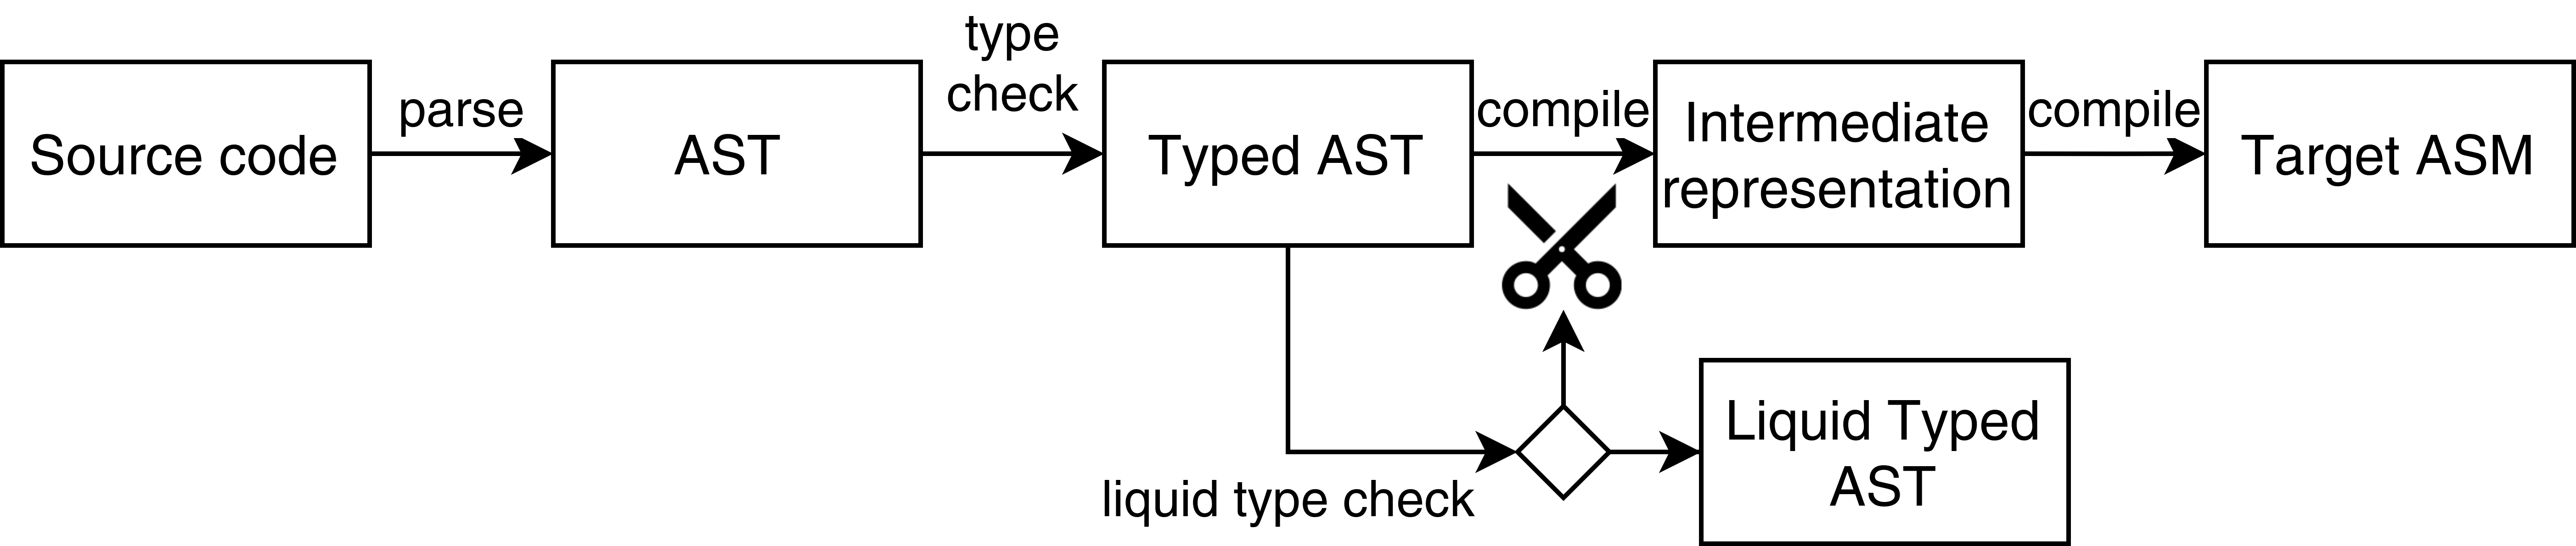
\includegraphics[scale=0.08]{hagia_pipeline}
\end{figure}

The implementation follows the algorithm proposed in Rondon's paper
\cite{liquid}, which is split into three main phases:

\subsubsection{Hindley--Milner type inference}

This step is already done by the Sophia type checker, so its details are not
discussed in this document. What is important, it returns an AST decorated with
type annotations on each node. This information shall serve for the liquid
typing initialisation in the next phase.

\subsubsection{Constraint generation}

The purpose of this process is to upgrade the types inferred in the previous
step to their liquid equivalents, and define constraints that must hold in order
to make the liquid typing valid. The generated constraints reflect dependencies
between types and assert assumptions about the control flow. Some constraints
are fixed, such as these explicitly given by the user, and some are yet unknown
and are subject to the weakening in the next step.

\subsubsection{Constraint solving and iterative weakening}

This is the process of satisfying the constraints. They are iteratively checked
for validity and if it is not the case, the inference relaxes the ones that can
be adjusted, until the system is consistent. If it manages to converge to a
point where every constraint is satisfied, a liquid typing is returned.
Otherwise, an error is reported.

\section{Used technology}

As the existing Sophia compiler is written in Erlang, it is most convenient to
use a programming language that also runs on the Open Telecom Platform
\cite{ericssonab2021}. Of such languages, Erlang and Elixir seem to be the most
mature and since the latter requires some additional effort for inter-operating
with the current implementation, the former was chosen.

During constraint solving the help of an SMT solver is invaluable, so following
Rondon's implementation of liquid types, Z3 by Microsoft Research
\cite{10.1007/978-3-540-78800-3_24} was chosen. Among many of its advantages,
the most convincing is the support of the SMT-lib language and a wide variety of
theories and abstractions that are useful for expressing judgements about the
values in Sophia. Furthermore, its performance has been proven to excel by
numerous successes at SMT-COMP competitions.

\section{Preprocessing}

Before the main algorithm is executed, the AST needs to be stripped of certain
abstractions. This is mostly due to the fact that the solving utility accepts
only a tight range of expressions, and it is much more convenient to analyse
simpler code and in a more selective manner. Therefore, several preprocessing
techniques are introduced.

\subsection{$\alpha$-normalisation}

\begin{defi}
  An expression is in the $\alpha$-normal form if it has no subexpressions that
  introduce variables which are already bound in their context.
\end{defi}

$\alpha$-normalisation is therefore a process of elimination of variable
shadowing. It can be done by performing subsequent $\alpha$-conversions
\cite{alpha_norm}, although in Hagia an error is thrown if a name collision is
detected. This is because shadowing can lead to hard to detect bugs if both
variables have the same type.

Without this process certain dependencies would become malformed or impossible
to express. Consider the following code:

\begin{minipage}{\linewidth}
\begin{lstlisting}[language=sophia]
let x = 1
let x = x + x  // this is not recursive
x
\end{lstlisting}
\end{minipage}

There is a collision on $x$ which can effectively confuse the solver; it would
receive an assertion that $x = 1 \land x = x + x$ which is not satisfiable. In
fact, the former $x$ and the latter one are different variables and thus have to
be reffered with different names. $\alpha$-normalisation is there to fix it by
appriopriate renaming:

\begin{minipage}{\linewidth}
\begin{lstlisting}[language=sophia]
let x_0 = 1
let x_1 = x_0 + x_0
x_1
\end{lstlisting}
\end{minipage}

\subsection{A-normalisation}

A-normalisation simplifies code by unpacking certain compound expressions and
explicitly assigning their parts to variables \cite{10.1145/173262.155113}. Most
often, its purpose is to reduce the gap between high-level abstract programs and
their lower-level representations. An accurate definition has been proposed by
Matt Might in one of his articles \cite{a_norm}:

\begin{quote}
  \begin{defi}
    An expression is atomic if:

    \begin{itemize}
    \item it is guaranteed to terminate;
    \item it causes no side effects;
    \item it causes no control effects; and
    \item it never produces an error.
    \end{itemize}
  \end{defi}

  \begin{defi}
    In A-Normal Form, all non-atomic (complex) expressions must be let-bound, or
    else appear in tail position.
  \end{defi}
\end{quote}

For instance, the following code

\begin{minipage}{\linewidth}
\begin{lstlisting}[language=sophia]
function factorial(n) =
  if(n == 0) 1
  else factorial(n - 1) * n
\end{lstlisting}
\end{minipage}

would be converted to

\begin{minipage}{\linewidth}
\begin{lstlisting}[language=sophia]
function factorial(n) =
  let b = n == 0
  if(b) 1
  else
    let v1 = n - 1
    let v2 = factorial(v1)
    v2 * n
\end{lstlisting}
\end{minipage}

Code in this form is much more convenient to analyse because every non-jumping
intermediate expression is named. This provides the refiner with handles to all
necessary parts of the program, allowing it to refer them independently. The
semantics are entirely preserved during A-normalisation.

\subsection{Purification}

This step is unavoidable due to the impure nature of Sophia, which does not
weave into Rondon's algorithm very well. Furthermore, mutable state is not
supported by the purely declarative SMT solver language. As stated in the
\autoref{chapter_sophia}, smart contracts do process an explicit mutable state
along with some additional variable properties like balances, remaining gas and
so on. This applies not only to the main contract, but also remote ones. Thus,
the aim is to convert the code to an equivalent one which is free of these
mechanisms.

Purification is the most convenient to perform on already A-normalised code due
to the assumption of purity of all sub-expressions in non-tail positions. This
vastly reduces the cases to cover, as it is no longer needed to check if, for
example, arguments in a function application interfere with the state. The
process does not need to preserve the A-normal form though. Since the
A-normalisation process does not affect the purity, it can be triggered once
again after the purification.

The expected outcome should resemble the \texttt{State} monad
\cite{markp.jones1995} pattern, where each function is additionally
parameterised by an argument representing the incoming state of computation and,
if it is stateful, modified to return the new state aside from the original
result. A similar approach is applied to the built-in statements that are
identified to be impure. This way the system keeps track of the changes by
making subsequent stateful operations introduce new variables representing
different stages of the chain state.

For the purpose of this algorithm the \texttt{chain\_state} is introduced. It
encapsulates everything related to the blockchain that might be altered during
the execution. In the current implementation, it is limited to two variables:

\begin{itemize}
\item \texttt{state} --- for tracking the internal state of the contract
\item \texttt{balance} --- for tracking the balance of the contract
\end{itemize}

This list can be further extended, if there is a need for a more detailed view
on the interaction with the chain. For convenience, handles of these values can
be stored in a dedicated \texttt{record} type and passed along with the control
flow. Although, Hagia keeps them separated to simplify the process of constraint
generation.

The purification process is itself stateful as it needs to keep the most actual
state reference and update it as needed. In case of Sophia, there are actually
not many primitive operations which are impure; thanks to the A-normalisation,
the only cases that are needed to be treated specially are:

\begin{itemize}
\item \texttt{state} --- should be replaced with the variable representing the
  current state reference.
\item \texttt{put} --- replaced with \texttt{()} and the state reference is set
  to the argument.
\item \texttt{Chain.spend} --- sets the balance variable to the previous one
  reduced by the sent amount. The expression has to be again typed as a
  non-negative integer.
\item \texttt{Contract.balance} --- replaced with the balance variable.
\item Remote contract calls --- the function call should be kept so the return
  value can be computed (possibly with an updated liquid type of
  \texttt{Call.value}, if the refinement system handles it). If the call value
  is set, then it should be subtracted from the balance before the call,
  similarly to the \texttt{Chain.spend}. Furthermore, the initial balance of the
  called contract can be safely assumed to be greater or equal to the sent
  value.
\item Stateful function calls --- since they may modify the state, they should
  return a tuple with the updated state and the actual return value.
\item Calls by a variable --- there is no control if the underlying function is
  stateful or not, so it is better to assume it is.
\item Calls to higher order functions --- if there is an argument which may be a
  stateful function, then the higher-order function should be considered
  stateful as well.
\item Oracle and AENS specific utilities --- if these object can be subjects of
  refinement, they should be handled appropriately. Current implementation of
  Hagia does not consider them, however.
\end{itemize}


The resulting code should be entirely pure and independent of these operations.
The semantics shall be preserved only in the purely computational sense --- the
outcome shall not be actually suited to interact with the blockchain, but rather
represent a more high-level view on the execution.
\autoref{example_before_purification} and \autoref{example_after_purification}
present examples of code before and after purification, respectively.

\begin{code}[h]{lexers/sophia.py:SophiaLexer -x}{Code before purification}{example_before_purification}
type state = int

stateful entrypoint f : () => address
entrypoint g : int => int

stateful entrypoint example(amount : int) : int =
  let addr = f()
  Chain.spend(addr, amount)
  put(amount)
  g(Chain.balance)
\end{code}

\begin{code}[h]{lexers/sophia.py:SophiaLexer -x}{Code after purification}{example_after_purification}
record chain_state =
  { state    : int,
    balance  : {b : int | b >= 0} }

entrypoint f : (chain_state) => chain_state * address
entrypoint g : (chain_state, int) => int

entrypoint example(cs0 : chain_state, amount : int) : chain_state * int =
  let (cs1, addr) = f(cs0)
  let cs2 = cs1{balance = cs1.balance - amount}
  let cs3 = cs2{state = amount}
  (cs3, g(cs3, cs3.balance))
\end{code}

In the examples, the stateful entrypoint \texttt{f} has been extended with an
additional argument carrying the representation of the incoming chain state and
modified to return the updated version of it. On the other hand, while
\texttt{g} also receives the chain state, its return value remains the same,
because it is not stateful. The call to \texttt{f} updates the carried chain
state reference aside from assigning the original result value to the
\texttt{addr} variable. The further calls to \texttt{Chain.spend}, \texttt{put}
and \texttt{Chain.balance} behave accordingly.

\section{The $\Gamma^*$ environment}

The $\Gamma^*$ environment has been defined as an extension to the regular
$\Gamma$ environment by changing base types into their liquid equivalents, and
attaching an additional path predicate. In Hagia, however, there are some
further features arising from the properties of Sophia. Among them there are
scope handles, current namespace and a registry of stateful entrypoints.
Moreover, for the purpose of the initial assignment algorithm described in the
\autoref{initial_assignment}, a collection of potentially relevant integers is
stored.

\section{Constraint generation}

This phase does not perform any verification itself, but rather defines a number
of statements that must hold in certain environments. Aside from that, it is
similar to the regular type checking as it computes a liquid typing for the
provided typed AST.

There are four kinds of such constraints:
\begin{itemize}
\item \emph{Well-formed} constraint which indicates existence of a liquid type,
  ensuring that it is properly initialised and the assigned qualifiers are
  correctly typed in a given environment. Denoted by $\Gamma^* \vdash \tau$
  where $\Gamma^*$ is the environment and $\tau$ is a well-formed type.
\item \emph{Subtype} constraint which asserts that some type is a subtype of
  another in a certain environment. Described using $\Gamma^* \vdash \tau_{sub}
  <: \tau_{sup}$ meaning that $\tau_{sub}$ is a subtype of $\tau_{sup}$ in
  $\Gamma^*$.
\item \emph{Reachable} constraint which ensures that some environment has a
  chance of being visited.
\item \emph{Unreachable} constraint which indicates an invalid environment which
  must be proven never to occur.
\end{itemize}

Each of these describe certain promises that have to be fulfilled in order to
find a valid liquid typing. This section reviews the process of generating them
from a typed AST.

\subsection{Decorating types with logical qualifiers}

This operation turns a base type into a corresponding liquid one. As provided by
the syntax, the user can specify liquid types manually and these remain
unchanged. Otherwise, if a non-liquid type is detected, it is enhanced with an
appropriate refinement. Fresh predicates created in this phase are represented
by \emph{liquid templates} as described in Rondon's algorithm \cite{liquid}. A
liquid template consists of a \emph{liquid type variable} and a \emph{pending
  substitution}. The former serves as the identifier of a predicate to be
resolved. Each time a substitution is applied to a liquid template, it is
accumulated in the pending substitution instead of altering the underlying
predicate, so it will not affect other occurences of that type.

Since the aim is to infer as strong judgements as possible, the positions of
types must be taken into account during the initialisation. When a type
describes the output of some computation, like for example the result of a
function or a variable introduction, it is called \emph{covariant}. It should
receive the whole space of possible qualifications and be therefore decorated
with a fresh liquid template. Otherwise, if a type is on an input position, such
as a function argument or a map key, it is defined to be \emph{contravariant}.
In contrary to the covariant ones, these types receive empty qualifications
which put no restrictions on the inhabiting values. Consequently, simple types
are decorated as follows:

\begin{lstlisting}[language=pseudocode]
fresh_template(variance) =
    let predicate =
            if variance == Covariant then fresh_liquid_var()
            else $\top$
        subst = []
    return make_template(subst, predicate)

fresh_liquid_simple(variance, $\mathbb{T}$) = -- covers primitives and type vars
    return $\{\nu : \mathbb{T} | \text{fresh\_template(covariant)}\}$
\end{lstlisting}

More than that, the variance switches each time an input position is entered, so
an argument of a function which is an argument of a higher-order function shall
be covariant instead.

\begin{lstlisting}[language=pseudocode]
switch_variance(Covariant) = Contravariant
switch_vairance(Contravariant) = Covariant

fresh_liquid_fun(variance, args, ret) =
    let args1 = [ ($\{\text{arg} : \text{fresh\_liquid}(\text{switch\_variance(variance)}, \tau)\}$)
                | $\{\text{arg} : \tau\}$ $\leftarrow$ args]
        ret1 = fresh_liquid(variance, ret)
    return $\text{args1} \to \text{ret1}$
\end{lstlisting}

The intuition here is to start with the least possible knowledge, while leaving
an opportunity for learning new facts. Covariant types describe values that are
built up across the computation, so in order to represent full uncertainty the
refiner considers all possible properties which may or may not apply. In
contrast, there is no judgement to be put on the incoming values, as they do not
depend on the expression itself, but rather on its use in other contexts.
Because of this, the refiner must be prepared to receive anything in their place
and thus strip all the assumptions off.

The only exception to this rule are lists' length predicates, because one can be
always sure that they will never be negative. In this special case, they are
initialised to $\{\nu : \texttt{list(\_)} | \nu \geq 0\}$.

\begin{lstlisting}[language=pseudocode]
fresh_liquid_list(variance, elem_t) =
    let len_predicate =
            if variance == Covariant then fresh_liquid_var()
            else $\nu \geq 0$
        subst = []
        elem_lt = fresh_liquid(variance, elem_t)
    return $\{\nu : \text{list(elem\_lt)} | \text{make\_template(subst, len\_predicate)}\}$
\end{lstlisting}

\subsubsection{Example}

For a reference of what happens in this process, let us consider the type of the
\texttt{List.map} function from the standard library, that applies a function
over every element of a given list. Assuming that a function is the first
argument, the type inferred by the original type checker is $(\alpha \to \beta,
\texttt{list}(\alpha)) \to \texttt{list}(\beta)$, which after decoration is
changed to

$$(\{\texttt{x} : \alpha | \rho_1\} \to \{\nu : \beta | \top\},
\{\texttt{l} : \texttt{list}(\{\nu : \alpha | \top\}) | \texttt{l} \geq 0\}\})
\to \{\nu : \texttt{list}(\{\nu : \alpha | \rho_2\}) | \rho_3\}$$

Where $\rho_1$, $\rho_2$ and $\rho_3$ are fresh liquid templates and $\top$ is an
empty predicate. The return value of the incoming function has been initialised
with an empty predicate, because it is on a contravariant position. A similar
thing has happened to the input list and its elements, except that non-negative
length has been assumed. The argument of that function is back on a covariant
position, so, just like the return value of \texttt{List.map}, has received a
fresh liquid template. In the end, $\rho_1$ and $\rho_2$ are resolved to $\top$,
and $\rho_3$ turns into $\nu = l$ to express that \texttt{List.map} preserves
the length. If the programmer had specified the predicates under the liquid
templates explicitly, they would have been left unaltered.

\subsubsection{User-definable types}
\label{user_definable_types}

Type aliases are resolved and processed further down.

\begin{lstlisting}[language=pseudocode]
fresh_liquid_alias(variance, name) =
    return fresh_liquid(variance, solve_name(name))
\end{lstlisting}

The identifiers of records are expanded to expose their underlying definitions
and turned into their liquid equivalents.

\begin{lstlisting}[language=pseudocode]
fresh_liquid_record(variance, $\mathbb{T}$) =
    let fields1 = [($\text{field} : \text{fresh\_liquid}(\text{variance}, \tau)$) | ($\text{field} : \tau$) $\leftarrow$ $\mathbb{T}$.fields]
    return $\{\mathbb{T} <: \text{fields1}\}$
\end{lstlisting}

Variants are unfolded similarly to records, but there is one more thing specific
them; their user-facing representation follows the description specified in
\autoref{liquid_types}, but for constraint generation they need to be
preprocessed to simplify the splitting rules discussed in the
\autoref{sub:constraint_splitting}. As stated before, liquid variants restrict
their domains not only by using liquid types in parameters of constructors, but
also allow banishing whole constructors from defining the inhabiting values,
regardless of their arguments. In this phase these two roles are split by
redefining liquid variants to utilise all their constructors and keep separate
\emph{tag predicates} that assert that a given value may or may not have been
created using given constructor.

\begin{lstlisting}[language=pseudocode]
fresh_liquid_variant(variance, $\mathbb{T}$) =
    let constructors1 =
            [ constr([($\{\text{arg} : \text{fresh\_liquid}(\text{variance}, \tau)\}$) | $\{\text{arg} : \tau\}$ $\leftarrow$ args])
            | constr(args) $\leftarrow$ $\mathbb{T}$.constructors]
    return $\{\{\nu : \mathbb{T} | \text{fresh\_template(variance)}\} <: \text{constructors1}\}$
\end{lstlisting}

Tag predicates take form of a conjunction of (possibly negated) either equality
against nullary constructors or existential expressions stating that it is
possible to find such arguments, that applied to that constructor build a
well-typed value. Although Sophia does not support existential quantification,
these qualifications do not escape internals of the inference algorithm, so they
do not conflict with the syntax.

More than that, missing constructors in user-defined liquid variants have
their parameters restricted to their minimal subtypes. It essentially means that
each covariant argument is initialised with a single qualification $\bot$
(\texttt{false}) instead of a fresh template. This allows expressing subtyping
more accurately later on.

\begin{minipage}{\linewidth}
\begin{lstlisting}[language=pseudocode]
fresh_liquid_dep_variant(variance, $\mathbb{T}$, declared_constructors) =
    let all_constructors = $\mathbb{T}$.constructors
        names_declared = [constr | constr(args) $\leftarrow$ declared_constructors]
        names_all      = [constr | constr(args) $\leftarrow$ all_constructors]

        constructors_combined =
            [constr(args) | constr(args) $\leftarrow$ declared_constructors] +
            [constr(args) | constr(args) $\leftarrow$ all_constructors,
                            $\text{constr} \notin \text{names\_declared}$]

        constructors1 =
            [ constr([($\{\text{arg} : \text{fresh\_liquid}(\text{variance}, \tau)\}$) | $\{\text{arg} : \tau\}$ $\leftarrow$ args])
            | constr(args) $\leftarrow$ constructors_combined]
        is_not(constr, arity) =
            if arity == 0 then return $\nu \neq  \text{constr}$
            else return $\lnot(\exists \text{args}. \nu = \text{constr(*args)})$
        tag_pred =
            fold_left(($\land$), $\top$,
                [ is_not(constr, length(args))
                | constr(args) $\leftarrow$ all_constructors,
                  $\text{constr} \notin \text{names\_declared}$])

    return $\{\{\nu : \mathbb{T} | \text{tag\_pred}\} <: \text{constructors1}\}$
\end{lstlisting}
\end{minipage}

For example, let us consider a type defined as \texttt{datatype t = C1 | C2(int)
  | C3(int)} and its liquid subtype $\{\texttt{t} <: \texttt{C2}(\{\nu :
\texttt{int} | \nu > 0\})\}$. After decoration, it is restructured to
$$\{\{\nu : \texttt{t} | \nu \neq \texttt{C1} \land \lnot(\exists a_1. \nu =
\texttt{C3}(a_1))\} <: \texttt{C1} | \texttt{C2}(\{\nu : \texttt{int} | \nu >
0\}) | \texttt{C3}(\{\nu : \texttt{int} | \bot\})\}$$

That reads: ``a type of such $\nu : \texttt{t}$, that $\nu$ is not \texttt{C1}
nor can be constructed with \texttt{C3}, and if it is built with \texttt{C2}
then its parameter is greater than zero''. While being more complicated, it
explicitly describes the meaning of the former notation. Furthermore, the
falsified assumption on the parameter of \texttt{C3} causes the type
$\{\texttt{t} <: \texttt{C2}(\{\nu : \texttt{int} | \nu > 0\})\}$ to be a
subtype of $\{\texttt{t} <: \texttt{C2}(\{\nu : \texttt{int} | \nu > 0\}) |
\texttt{C3}(\{\nu : \texttt{int} | \bot\})\}$. Note that because of the tag
predicate the subtyping does not work the other way around --- please refer to
the \autoref{effective_variant_types} for the discussion.

\subsection{Preparing the environment}

Normally namespaces and contracts are processed in a way that allows mutual
recursion among the functions they contain, but not across the scopes. This does
not necessarily reflect the case of liquid inference, as the dependencies may
flow in both directions. Thus, before the functions' bodies are examined, all
signatures are refined and registered in the environment. Custom type
definitions have to be handled beforehand.

An important requirement that needs to be verified in this step is that no
entrypoint has assumptions on its input. This is crucial when user decides to
declare liquid types on their own, because none of the contravariant assertions
would actually be checked at runtime. Subsequently, the programmer might be
wrongfully convinced that the function is safe from receiving improper input.

Formally speaking, in all entrypoints' signatures, the contravariant types must
not be qualified by any logical statements that would exceed the guarantees made
by the virtual machine. The covariant ones are free of this restriction, because
they serve as ``promises'' of the contract, not ``expectations''. Note that
despite being theoretically an input of every function, the \texttt{state} value
always comes from inside of a contract and cannot be therefore set out-of-domain
by a malicious user. Because of that, it should be considered solely covariant
in this context.

\subsection{Constraining global functions}

For a given function $f$ we define its \emph{global type} $F_g$ derived from the
previous step, and its \emph{local type} $F_l$ which emerges from the constraint
generation of its body. The body is processed in the environment $\Gamma^*_a$,
which is extended by the arguments' bindings and the assertions that the
arguments from the definition and the type declaration are in fact the same
values.

Afterwards, appropriate constraints are produced. First, it is necessary to
assert that both $F_l$ and $F_g$ are well-formed. Next, there must be a
subtyping relation between $F_l$ and $F_g$, so the implementation fits the
declaration.

\subsubsection{Example}

For a simplistic example, let us consider a constant function that returns 1.
However, the programmer has specified its type just to return an integer that is
greater than 0. The function can be defined as follows:

\begin{minipage}{\linewidth}
\begin{lstlisting}[language=sophia]
function
  pos_int : () => {r : int | r > 0}
  pos_int() = 1
\end{lstlisting}
\end{minipage}

In this snippet, $F_l$ is inferred to be $() \to \{r : \texttt{int} | r =
1\}$ and $F_g$ is declared as $() \to \{r : \texttt{int} | r > 0\}$. The
subtyping relation between these types holds, making the program well-typed.
Details on how $F_l$ has been constructed are discussed in the
\autoref{ssec:constr_expr} in this chapter. The verification of the subtyping is
covered in the \autoref{sec:solving}.

\subsection{Constraining expressions}
\label{ssec:constr_expr}

Since Sophia has a very rich syntax, there are numerous cases to consider in
this step. Because of that, only the most principal, unique, or otherwise
interesting have been selected. Needless to say, many of the omitted cases can
be easily derived from the presented ones. For a broader view, please refer to
the original implementation in the GitHub repository.

\subsubsection{Variables}

Constraining variables depends on whether their type is simple enough to make
the equality assertion meaningful. In the original implementation
\texttt{is\_simple} is defined to check if the type is either a primitive or a
type variable. In such a case, an equality assumption provides as much
information as the current knowledge about the underlying value, but can be
expressed with just a single qualification instead. Otherwise, the original type
is inherited.

\begin{minipage}{\linewidth}
\begin{lstlisting}[language=pseudocode]
constr_expr_var($\Gamma^*$, name, type) =
    let ltype = fresh_liquid($\Gamma^*$, type)  -- solves aliases by the way
        baseT = base_type(ltype)  -- `type` is not guaranteed to be base
    if is_simple(baseT) then
        return $\{\nu : \text{type} | \nu = \text{name}\}$
    else
        return type_of($\Gamma^*$, name)
\end{lstlisting}
\end{minipage}

\subsubsection{Integer arithmetic}
\label{constr_expr_int}

The integer literal is one of the simplest cases, because every property of it
can be concluded directly from its known value.

\begin{lstlisting}[language=pseudocode]
constr_expr_int($\Gamma^*$, n) =
    return $\{\nu : \text{int} | \nu = \text{n}\}$
\end{lstlisting}

The arithmetic operations are typed in a way that allows the solver deriving the
information about their result directly from the operands. As an example, the
division has been chosen because it presents an additional requirement for the
right-hand value not being equal to 0.

\begin{lstlisting}[language=pseudocode]
constr_expr_op($\Gamma^*$, "/") =
    let opLV  = fresh_id()
        opRV  = fresh_id()
    return $(\{\text{opLV} : \text{int}\}, \{\text{opRV} : \text{int} | \text{opRV} \neq 0\}) \to \{\nu : \text{int} | \nu = \text{opLV} / \text{opRV}\}$
\end{lstlisting}

\subsubsection{Function application}

In Hindley--Milner, the type of a function application is inferred to be its
codomain. However, with liquid types it may vary depending on the values of the
arguments. Consequently, an appropriate substitution has to be applied. It can
be done directly due to the A-normalisation, which ensures that the arguments
are atomic and thus simple enough to be used in qualifiers. In order to ensure
that the application is valid, a proper subtyping relation must hold between the
declared and provided arguments. Therefore, for each pair $(a_i, \tau_i)$, where
$\tau_i$ is the type of the i-th argument from the function domain and $a_i$ is
the inferred type of the respective value, the $\Gamma^* \vdash a_i <: \tau_i$
constraint is produced.

\begin{lstlisting}[language=pseudocode]
constr_expr_app($\Gamma^*$, fun, argsApp) =
    let (argsFT $\to$ retT) = constr_expr($\Gamma^*$, fun)
        argsT = constr_exprs($\Gamma^*$, argsApp)
        argsSubst =
          [(argName, argVal) | ($\{\text{argName} : \_\}$, argVal) $\leftarrow$ zip(argsFT, argsApp)]

    for ($\{\_ : \text{argT}_\}$, argFT) in zip(argsT, argsFT) do
        constraint($\Gamma^* \vdash \text{argT} <: \text{argFT}$)
    return apply_subst(argsSubst, retT)
\end{lstlisting}

For example, considering an expression \texttt{4 / 2}, the system shall infer
the type $\{\nu : \texttt{int} | \nu = 4 / 2\}$ and generate the following
constraints:

\begin{align*}
  & \Gamma^* \vdash \{\nu : \texttt{int} | \nu = 4\} <: \{\nu : \texttt{int}\}\\
  & \Gamma^* \vdash \{\nu : \texttt{int} | \nu = 2\} <: \{\nu : \texttt{int} | \nu \neq 0\}
\end{align*}

While the first one does not introduce any useful information, the latter
asserts that there is no division by zero. Although the presented case is rather
trivial, this requirement would bring a lot of value if the right-hand operand
was a variable.

\subsubsection{\texttt{if} expression}

The \texttt{if} expression is one of the most representative examples of the
path predicate in use. First, the condition is processed, but only for the
purpose of constraints generation, as the type is already known to be boolean.
Then, the positive and negative cases are considered in $\Gamma^*$ with the path
predicate extended by the respective valuations of \texttt{cond} (the
\texttt{assert} function). In the end, the final type must be a supertype of
what has been inferred for both branches. The reachability constraints are
included to forbid dead code.

\begin{lstlisting}[language=pseudocode]
constr_expr_if($\Gamma^*$, cond, thenEx, elseEx, type) =
    constr_expr($\Gamma^*$, cond)
    let $\Gamma^*_t$ = assert(cond, $\Gamma^*$)
        $\Gamma^*_e$ = assert($\lnot$cond, $\Gamma^*$)
        thenT = constr_expr($\Gamma^*_t$, thenEx)
        elseT = constr_expr($\Gamma^*_e$, elseEx)
        $\tau$ = fresh_liquid($\Gamma^*$, type),
    constraint($\Gamma^* \vdash \tau$)
    constraint(reachable($\Gamma^*_t$))
    constraint(reachable($\Gamma^*_e$))
    constraint($\Gamma^*_t \vdash \text{thenT} <: \tau$)
    constraint($\Gamma^*_e \vdash \text{elseT} <: \tau$)
    return $\tau$
\end{lstlisting}

\subsubsection{Pattern matching}

Pattern matching is not covered in Rondon's work, so it is explained in more
details here. The very first step is to extract constraints from the desctructed
expression (the \texttt{switched} variable).

\begin{lstlisting}[language=pseudocode]
constr_expr_switch($\Gamma^*$, switched, alts, type) =
    let switchedT = constr_expr($\Gamma^*$, switched),
        $\tau$ = fresh_liquid($\Gamma^*$, type)
    constr_cases($\Gamma^*$, switched, switchedT, $\tau$, alts)
    constraint($\Gamma^* \vdash \tau$)
    return $\tau$
\end{lstlisting}

The alternatives are processed and combined into the return type similarly to
\texttt{if} branches, with the difference of using more advanced conditions,
additionally capable of introducing variables. Each alternative has its body
processed in the environment of a successful match to the current pattern along
with an assumption of failing matches in previous cases, as \texttt{switch}
considers the clauses top--down. An additional reachability constraint is
generated in order to disallow dead code. At the end, where no further
alternatives are available, the environment is asserted to be unreachable by a
relevant constraint. This prevents a pattern-exhaustion error and enforces the
programmer to consider all possible cases.

\begin{lstlisting}[language=pseudocode]
constr_cases($\Gamma^*$, switched, switchedT, returnT, alts) =
    if alts.non_empty() then
        let (pat $\implies$ val) = alts.first()
            ($\Gamma^*_+$, $\Gamma^*_-$) = match_to_pattern($\Gamma^*$, pat, switched, switchedT)
            valT = constr_expr($\Gamma^*_+$, val)
        constraint($\Gamma^*_+ \vdash \text{valT} <: \text{returnT}$)
        constraint(reachable($\Gamma^*_+$))
        constr_cases($\Gamma^*_-$, switched, switchedT, returnT, alts.drop_first())
    else constraint(unreachable($\Gamma^*$))
\end{lstlisting}

The split of the environments is done by the \texttt{match\_to\_pattern}
function. The auxiliary \texttt{match\_to} procedure builds up a predicate
describing a successful match and an environment in which all pattern variables
are bound. With this information, \texttt{match\_to\_pattern} creates a
succeeding environment with the assumptions applied and a failing one with no
new variables, but with the negation of the predicate asserted.

\begin{lstlisting}[language=pseudocode]
match_to_pattern($\Gamma^*$, pat, expr, type) =
    let ($\Gamma^*_m$, pred) = match_to($\Gamma^*$, pat, expr, type, $\top$)
        $\Gamma^*_+$ = assert(pred, $\Gamma^*_m$)
        $\Gamma^*_-$ = assert($\lnot$ pred, $\Gamma^*$)
    return ($\Gamma^*_+$, $\Gamma^*_-$)
\end{lstlisting}

During the predicate build-up there are three main kinds of patterns:
\begin{itemize}
\item Literal patterns --- for example integers. They extend the matching
  predicate by an assumption that the destructed expression has a given
  value.
\item Variables --- these do not add anything to the matching predicate, but
  instead extend the environment with an appropriate variable binding.
\item Complex patterns --- for example tuples or lists. They require unpacking
  the component data and sometimes verifying the general form of the destructed
  value. In case of a tuple, the pattern matching proceeds by matching the
  projections against the respective sub-patterns. In case of variant types, an
  additional constructor tag assertion is added. Lists introduce mock
  \texttt{int} variables which derive their qualifications from length
  predicates and are asserted to imply the value induced by the pattern.
\end{itemize}

It is assumed that \texttt{match\_to} splits over possible kinds of patterns and
dispatches across functions as such:

\begin{minipage}{\linewidth}
\begin{lstlisting}[language=pseudocode]
match_to_var($\Gamma^*$, name, expr, type, pred) =
  return (bind_var(name, type, $\Gamma^*$), pred)

match_to_int($\Gamma^*$, n, expr, type, pred) =
  return ($\Gamma^*$, $\text{expr} = \text{n} \land \text{pred}$)

match_to_tuple($\Gamma^*$, pats, patsT, expr, pred) =
    return fold_left(
      fun(($\Gamma^*_1$, pred_1), (pat, patT, idx)) $\to$
           return match_to_pattern($\Gamma^*_1$, pat, expr[idx], patT, pred_1)
      end,
      ($\Gamma^*$, pred),
      zip(pats, patsT, [1..length(pats)])
    )
\end{lstlisting}
\end{minipage}

To visualise the process, let us consider a simple pattern matching shown in the
code snippet below:

\begin{lstlisting}[language=sophia]
function f(m : option(int)) : int =
  switch(m)
    None => 1
    Some(0) => 1
    Some(n) => n
\end{lstlisting}

The constraints are generated as follows:

\begin{enumerate}
\item First, the destructed expression \texttt{m} comes with a (redundant in
  this case) well-formedness constraint on its type:
  $$\Gamma^* \vdash \texttt{option(int)}$$.
\item The overall return type is declared to be well-formed:
  $$\Gamma^* \vdash \tau$$
\item In the first alternative, \texttt{m} is matched against a 0-arity
  constructor \texttt{None}. Hence, the following constraint is created to
  assert that, if the match succeeds, the result fits in the return type
  $\tau$ (created in the previous step):
  $$\Gamma^*, \texttt{m} = \texttt{None} \vdash \{\nu : \texttt{int} | \nu = 1\}
  <: \tau$$ Besides that, the refiner requires this case to be
  achievable:
  $$\texttt{reachable}((\Gamma^*, \texttt{m} = \texttt{None}))$$
\item The second alternative is triggered when the previous case has failed,
  \texttt{m} is \texttt{Some} and it wraps 0. If all these hold, the result is
  again 1. A negated matching predicate from the \texttt{None} case is attached
  to the path predicate of $\Gamma^*$ to express the first condition, even
  though it is actually redundant here. The \texttt{m\_unwrap} variable is
  introduced as a handle to the value under the \texttt{Some} constructor.
  \begin{align*}
    & \Gamma^*, \texttt{m\_unwrap} : \texttt{int}, \lnot(\texttt{m} = \texttt{None}), \texttt{m\_unwrap} = 0, \texttt{m} = \texttt{Some(m\_unwrap)} \vdash\\
    & \{\nu : \texttt{int} | \nu = 1\} <: \tau\\
    & \\
    & \texttt{reachable}((\Gamma^*, \texttt{m\_unwrap} : \texttt{int}, \lnot(\texttt{m} = \texttt{None}), \texttt{m\_unwrap} = 0, \texttt{m} = \texttt{Some(m\_unwrap)}))
  \end{align*}
\item For the third alternative to be visited, the previous ones must have
  failed the match and the constructor of \texttt{m} needs to be \texttt{Some}.
  Then a new variable \texttt{n} is introduced and assigned to the value wrapped
  by \texttt{m}. The generated constraints are therefore:
  \begin{align*}
    & \Gamma^*, \texttt{m\_unwrap} : \texttt{int}, \lnot(\texttt{m} = \texttt{None}), \lnot(\texttt{m\_unwrap} = 0 \land \texttt{m} = \texttt{Some(m\_unwrap)}),\\
    & \texttt{n} : \{\nu : \texttt{int} | \nu = \texttt{m\_unwrap}\}, \texttt{m} = \texttt{Some(n)} \vdash\\
    & \{\nu : \texttt{int} | \nu = 1\} <: \tau \\
    & \\
    & \texttt{reachable}((\Gamma^*, \texttt{m\_unwrap} : \texttt{int}, \lnot(\texttt{m} = \texttt{None}), \lnot(\texttt{m\_unwrap} = 0 \land \texttt{m} = \texttt{Some(m\_unwrap)}), \\
    & \phantom \quad \texttt{n} : \{\nu : \texttt{int} | \nu = \texttt{m\_unwrap}\}, \texttt{m} = \texttt{Some(n)}))
  \end{align*}
\item Last, the \texttt{switch} expression is disallowed to have its patterns
  exhausted. Thus, the final constraint is generated as follows:
  \begin{align*}
    & \texttt{unreachable}((\Gamma^*, \texttt{m\_unwrap} : \texttt{int}, \lnot(\texttt{m} = \texttt{None}),
      \lnot(\texttt{m\_unwrap} = 0 \land \texttt{m} = \texttt{Some(m\_unwrap)}),\\
    & \phantom \quad \texttt{n} : \{\nu : \texttt{int} | \nu = \texttt{m\_unwrap}\}, \lnot(\texttt{m} = \texttt{Some(n)})))
  \end{align*}
\end{enumerate}

\subsection{Constraint splitting}
\label{sub:constraint_splitting}

The generated constraints may now consist of complex types which require an
additional decomposing logic for their validation. This logic can be in fact
applied just once as an intermediate step before the solving phase. Thus, the
aim is to reduce the number of cases to only those involving base types with
logical refinements by splitting the compound ones into parts.

This subsection describes the splitting algorithm only for the subtyping
contraints, because the strategy for well-formedness is very similar and neither
reachability nor unreachability require splitting. Moreover, assuming the
correctness of the previous phases, the only cases that are to be examined here
are the ones in which every subtyping assertion is set between liquid types
of the same form. Therefore, the splitting algorithm goes as follows:

\subsubsection{Liquid types}

For two logically qualified types there is nothing to do since they are already
in their simplest form.

\begin{lstlisting}[language=pseudocode]
split_sub(constraint = $\Gamma^* \vdash \{\nu_{sub} : \mathbb{B} | \rho_{sub}\} <: \{\nu_{sup} : \mathbb{B} | \rho_{sup}\}$) =
    return [constraint]
\end{lstlisting}

\subsubsection{Functions}

For liquid function types $T_{sub} = \texttt{args}_{sub} \to \texttt{ret}_{sub}$
and $T_{sup} = \texttt{args}_{sup} \to \texttt{ret}_{sup}$ where $\Gamma^* \vdash
T_{sub} <: T_{sup}$ the splitting continues recursively on $\Gamma^*,
\texttt{args}_{sub} \vdash \texttt{ret}_{sub} <:
\texttt{ret}_{sup}[\texttt{args}_{sup} / \texttt{args}_{sub}]$ and
$\texttt{args}_{sup} <: \texttt{args}_{sub}$ (for each argument respectively).
Note the subtyping relation is swapped on \texttt{args} due to the variance
switch when entering types on contravariant positions. To make the subtyping of
the codomains properly defined, the environment takes the arguments into account
and unifies them between both sides by applying a proper substitution.

\begin{lstlisting}[language=pseudocode]
split_sub($\Gamma^* \vdash \text{args}_{sub} \to \text{ret}_{sub} <: \text{args}_{sup} \to \text{ret}_{sup}$) =
    let args_constrs =
             [ constr
             | $(\{\text{arg}_{sub} : \tau_{sub}\}, \{\text{arg}_{sub} : \tau_{sub}\}) \leftarrow \text{zip}(\text{args}_{sub}, \text{args}_{sup})$,
               constr $\leftarrow$ split_sub($\Gamma^* \vdash \tau_{sup} <: \tau_{sub}$)]
        $\Gamma^*_r$ = bind_args($\text{args}_{sup}$, $\Gamma^*$)
        subst = [$(\text{arg}_{sub}, \text{arg}_{sup})$ | $(\{\text{arg}_{sub} : \tau_{sub}\}, \{\text{arg}_{sub} : \tau_{sub}\}) \leftarrow \text{zip}(\text{args}_{sub}, \text{args}_{sup})$]
    return args_constrs + split_sub($\Gamma^*_r \vdash \text{apply\_subst}(\text{subst}, \text{ret}_{sub}) <: \text{ret}_{sup}$)

\end{lstlisting}

For example
\begin{align*}
  & \Gamma^* \vdash \{x : \texttt{int} | x > 0\} \to \{\nu : \texttt{int} | \nu >
    x\} <: \{y : \texttt{int} | y = 1\} \to \{\nu : \texttt{int} | \nu \geq y\}
\end{align*}

is split into

\begin{align*}
  & \Gamma^* \vdash \{x : \texttt{int} | x > 0\} <: \{y : \texttt{int} | y = 1\}\\
  & \Gamma^*, x : \{\nu : \texttt{int} | \nu > 0\} \vdash \{\nu : \texttt{int} | \nu >
    x\} <: \{\nu : \texttt{int} | \nu \geq x\}
\end{align*}

\subsubsection{Records and tuples}

Record types and tuples are split element-wise. Here only pairs are presented,
as other cases are handled similarly.

\begin{lstlisting}[language=pseudocode]
split_sub($\Gamma^* \vdash \tau^l_{sub} \times \tau^r_{sub} <: \tau^l_{sup} \times \tau^r_{sup}$) =
    let constr_l = split_sub($\Gamma^* \vdash \tau^l_{sub} <: \tau^l_{sup}$)
        constr_r = split_sub($\Gamma^* \vdash \tau^r_{sub} <: \tau^r_{sup}$)
    return constr_l + constr_r
\end{lstlisting}

For example
\begin{align*}
  & \Gamma^* \vdash \{\nu : \texttt{int} | \nu > 0\} * \{\nu : \texttt{int} | \nu < 1\} <: \{\nu : \texttt{int} | \nu \geq 0\} * \{\nu : \texttt{int} | \nu \leq 1\}
\end{align*}

is split into

\begin{align*}
  & \Gamma^* \vdash \{\nu : \texttt{int} | \nu > 0\} <: \{\nu : \texttt{int} | \nu \geq 0\}\\
  & \Gamma^* \vdash \{\nu : \texttt{int} | \nu < 1\} <: \{\nu : \texttt{int} | \nu \leq 1\}
\end{align*}

\subsubsection{Variants}

Variant types are split on the arguments of their constructors element-wise and
emit additional liquid types for keeping the tag predicates.

\begin{lstlisting}[language=pseudocode]
split_sub($\Gamma^* \vdash \{\{\nu : \mathbb{T} | \rho_{sub}\} <: \text{cs}_{sub} \} <: \{\{\nu : \mathbb{T} | \rho_{sup}\} <: \text{cs}_{sup} \}$) =
    let from_constructors =
        [ constr
        | $(\text{constr}(\text{args}_{sub}), \text{constr}(\text{args}_{sup}))$ $\leftarrow$ zip(sort($\text{cs}_{sub}$), sort($\text{cs}_{sup}$)),
          $(\text{arg}_{sub}, \text{arg}_{sup})$ $\leftarrow$ zip($\text{args}_{sub}$, $\text{args}_{sup}$),
          constr $\leftarrow$ split_sub($\Gamma^* \vdash \text{arg}_{sub} <: \text{arg}_{sup}$)
        ]
    return [$\Gamma^* \vdash \{\nu : \mathbb{T} | \rho_{sub}\} <: \{\nu : \mathbb{T} | \rho_{sup}\}$] + from_constructors
\end{lstlisting}

For example

\begin{align*}
  & \Gamma^* \vdash t_1 <: t_2 \text{ where}&\\
  & t_1 = \{\{\nu : \texttt{option(int)} | \nu \neq \texttt{None}\} & <: \texttt{None} | \texttt{Some}(\{\nu : \texttt{int} | \nu > 0\})\}\\
  & t_2 = \{\{\nu : \texttt{option(int)} | \top\} & <: \texttt{None} | \texttt{Some}(\{\nu : \texttt{int} | \nu \geq 0\})\}
\end{align*}

is split into

\begin{align*}
  & \Gamma^* \vdash \{\nu : \texttt{int} | \nu > 0\} <: \{\nu : \texttt{int} | \nu \geq 0\}\\
  & \Gamma^* \vdash \{\nu : \texttt{option(int)} | \nu \neq \texttt{None}\} <: \{\nu : \texttt{option(int)} | \top\}
\end{align*}

\subsubsection{Lists}

Liquid lists split into subtyping on the element types and liquid integer types
with qualifications gained from the length predicates.

\begin{lstlisting}[language=pseudocode]
split_sub($\Gamma^* \vdash \{\nu : \text{list}(\tau_{sub}) | \rho_{sub}\} <: \text{list}(\tau_{sup}) | \rho_{sup}\}$) =
    return [$\Gamma^* \vdash \{\nu : \text{int} | \rho_{sub}\} <: \text{int} | \rho_{sup}\}$, $\Gamma^* \vdash \tau_{sub} <: \tau{sup}$]
\end{lstlisting}

For example
\begin{align*}
  & \Gamma^* \vdash \{\nu : \texttt{list}(\{\nu_e : \texttt{int} | \nu_e > 10\}) | \nu > 1\} <: \{\nu : \texttt{list}(\{\nu_e : \texttt{int} | \nu_e > 5\}) | \nu > 0\}
\end{align*}

is split into

\begin{align*}
  & \Gamma^* \vdash \{\nu_e : \texttt{int} | \nu_e > 10\} <: \{\nu_e : \texttt{int} | \nu_e > 5\}\\
  & \Gamma^* \vdash \{\nu : \texttt{int} | \nu > 1\} <: \{\nu : \texttt{int} | \nu > 0\}
\end{align*}

\section{Solving}
\label{sec:solving}

Having constraints generated across the AST, the final task is to find
predicates for each liquid variable, which, after substitution, satisfy the
constraints and yield the strongest possible guarantees. The heart of this
algorithm is the \emph{iterative weakening} which reduces the initial predicates
until a consistent model is found.

\subsection{Initial assignment}
\label{initial_assignment}

A \emph{liquid assignment} $\mathbb{A}$ is a map from liquid type variables to
predicates. For convenience, information about the base type and the value
handle identifier is stored there as well. Initially, for each variable a wide
space of logical sentences is provided --- it does not matter if these sentences
are contradictory or make any sense at that point. Ideally it would be defnined
with all possible logical expressions that involve that variable, but it is much
easier and most often sufficient to start with a finite, pre-defined set of
qualifiers.

Practically, this is the point where the well-formedness constraints do their
role. As they contain information about base types and the environments at the
time of their creation, it is possible to select qualifications that are
well-typed and somehow relevant. Depending on what the base type is, the
following strategies are taken:

\begin{itemize}
\item For integers it is useful to apply all known comparison operators to other
  \texttt{int} variables and list lengths in the context, as well as the integer
  literals that have been found in the surrounding expressions. Arithmetic
  operations may additionally generate many valuable samples. It is important to
  keep in mind that the number of generated qualifiers will affect the
  performance, but on the other hand will enhance the expressiveness of the
  inference. Nevertheless, it is almost always worth including comparison with 0
  and 1.
\item Booleans should have a chance to be proven both true and false and also
  depend on comparisons of same-typed values from the context. Again, the
  greater space the lower performance, but possibly better conclusions.
\item Lists are treated similarly to integers.
\item Variables for variant tags should be compared by equality and inequality
  with all of their possible constructors and values of the same type from the
  environment.
\item Type variables should be initialised with just equality and inequality
  with other values of their types.
\end{itemize}

Example implementation of initialisation of refined integers:

\begin{lstlisting}[language=pseudocode]
init_assg(constraints) =
    var $\mathbb{A}$ = Map.new()
    for constr = $\Gamma^* \vdash \mathbb{T}$ in constraints
        $\mathbb{A}$ := init_assg_1($\mathbb{A}$, constr)
    end
    return $\mathbb{A}$

init_assg_1($\mathbb{A}$, $\Gamma^* \vdash \{\nu : \text{int} | (\kappa . \theta)\}$) =
    let ints = [1, 0] + $\Gamma^*$.ints_so_far
        int_vars = [$x$ | $x : \tau$ $\leftarrow$ $\Gamma^*$.var_env, $\tau = \text{int} \lor \tau = \text{list(\_)}$]
    return [ 'bool_op($\nu$, r)
           | x $\leftarrow$ ints + int_vars,
             y $\leftarrow$ ints + int_vars,
             int_op $\leftarrow$ [($+$), ($-$)]
             r $\leftarrow$ 'int_op(x, y)
             bool_op $\leftarrow$ [($=$), ($\neq$), ($>$), ($<$), ($\geq$), ($\leq$)]
           ]
\end{lstlisting}

\subsection{Iterative weakening}

At this point the assignment map should be filled with possibly mutually
contradictory, unjustified and seemingly random statements. The aim of this
operation is to iteratively remove those that break the subtyping constraints
and find a consistent model that describes the properties of the program as
precisely as it can be expressed.

The algorithm consists of two parts: validity checking and predicate weakening.
In each step it verifies if the system is already consistent using the
\texttt{is\_valid} function. If that is the case, the solving is finished and
the most recent assignment is returned as the solution. If an invalid constraint
is found, the \texttt{weaken} function is called to adjust the predicates under
related liquid variables by removing qualifications that falsify the constraint.
Then, the whole operation is repeated from the beginning with the new
assignment.

\begin{lstlisting}[language=pseudocode]
solve(constraints) =
    var $\mathbb{A}$ = init_assg(constraints)
    while Some(c) = constraints.find(fun(c) not is_valid($\mathbb{A}$, c) end)
        $\mathbb{A}$ := weaken($\mathbb{A}$, c)
    end
    return $\mathbb{A}$
\end{lstlisting}

At this point, this process considers only subtyping constraints.
Well-formedness does not need validation, as the assignment has been initialised
in a way that guarantees that the predicates are not ill-typed. Reachability and
unreachability may break, but they can be verified once the subtyping is
resolved, because they do not contribute to the weakening process.

Note that it does not necessarily prevent contradictions from occuring in the
inferred qualifications. If a constraint was created in a contradictory
environment or describes a looping or crashing computation, it will induce false
assumptions and therefore false conclusions. Thus, variables typed in such a way
indicate computations without results.

The produced assignment should make all the well-formedness and subtype
constraints hold. The last thing to check is that all reachability and
unreachability constraints have been defined under satisfiable or unsatisfiable
assumptions respectively. This effectively means validating the path predicates
of their environments.

\subsubsection{Validtity checking and weakening}

Subtyping constraints can be divided into two categories. A constraint $\Gamma^*
\vdash \{\nu : T | \mathbb{P}_{sub}\} <: \{\nu : T | \mathbb{P}_{sup}\}$ is
defined as \emph{wobbly} if $\mathbb{P}_{sup}$ is a liquid template, and can
therefore be a subject of weakening. Otherwise, that is when $\mathbb{P}_{sup}$
is a fixed predicate, it is called \emph{rigid}. The main difference between
these two is that the first one is flexible and may be adjusted in case it
breaks the assumptions. The latter, on the contrary, serves as a strict
assertion that results in an error if not satisfied. It appears when the
supertype is placed on a contravariant position, or has been explicitly
qualified by the user.

For a subtyping constraint to be valid, the refiner must ensure that each value
of the subtype inhabits the supertype as well. For that to hold in the case of a
liquid type, the qualification of the supertype must be entirely derivable from
the subtype's. Formally said, a constraint $\Gamma^* \vdash \{\nu_{sub} : T |
\mathbb{P}_{sub}\} <: \{\nu_{sup} : T | \mathbb{P}_{sup}\}$ is valid if and only
if $\Gamma^* \vdash \mathbb{P}_{sub} \implies
\mathbb{P}_{sup}[\nu_{sup}/\nu_{sub}]$ which can be verified by the SMT solver.
The subtyping relation on base types has been already handled by the
Hindley--Milner inference at this point\footnote{In the 5.0.0 version of Sophia
  there is no actual subtyping, so in fact it is enough to check if the types
  unify.}. The checking algorithm goes as follows:

\begin{lstlisting}[language=pseudocode]
pred_of($\mathbb{A}$, $(\kappa . \theta)$) =
    return apply_subst($\theta$, $\mathbb{A}(\kappa)$)
pred_of($\mathbb{A}$, $\mathbb{P}$) =
    return $\mathbb{P}$

-- Wobbly
is_valid($\mathbb{A}$, $\Gamma^* \vdash \{\nu_{sub} : \mathbb{B} | \rho_{sub}\} <: \{\nu_{sup} : \mathbb{B} | \rho_{sup} = (\kappa . \theta)\}$) =
    let $\mathbb{P}_{sub}$ = pred_of($\mathbb{A}$, $\rho_{sub}$)[$\nu_{sub} / \nu_{sup}$]
        $\mathbb{P}_{sup}$ = pred_of($\mathbb{A}$, $\rho_{sup}$)
        $\Gamma^*_1$ = bind_var($\nu_{sup}$, $\mathbb{B}$, $\Gamma^*$)
    return SMT.holds($\mathbb{P}_{sub} \implies \mathbb{P}_{sup}$)
-- Rigid
is_valid($\mathbb{A}$, $\Gamma^* \vdash \{\nu_{sub} : \mathbb{B} | \rho_{sub}\} <: \{\nu_{sup} : \mathbb{B} | \mathbb{P}_{sup}$) =
    let $\mathbb{P}_{sub}$ = pred_of($\mathbb{A}$, $\rho_{sub}$)[$\nu_{sub} / \nu_{sup}$]
        $\Gamma^*_1$ = bind_var($\nu_{sup}$, $\mathbb{B}$, $\Gamma^*$)
    if SMT.holds($\Gamma^*$, $\mathbb{P}_{sub} \implies \mathbb{P}_{sup}$) then return true
    else error("Contradiction")
\end{lstlisting}

In order to fix an invalid wobbly constraint, the predicate of the supertype
needs to be weakened to make the above implication hold. Let us assume that
$\mathbb{P}_{sup}$ appears as a liquid template with $\kappa_{sup}$ as the
liquid variable and $\theta$ as the pending substitution. Thus, in line with the
previous notation, the weakened predicate under $\kappa_{sup}$ should be
redefined as

$$\{q | q \leftarrow \mathbb{A}[\kappa_{sup}], \Gamma^* \vdash \mathbb{P}_{sub} \implies q . \theta\}$$.

A key observation showing the correctness of this step is that predicates under
liquid variables can only grow weaker. Therefore, if some qualifiers cannot be
proven at one point, they will not be derivable later as well. Because of that,
it is fine to remove them from the predicate as soon as they break the
implication.

To visualise this mechanism, let us consider an expression \texttt{if(x == 0)
  2137 else 1 / x}. Among others, the following constraints should be
produced:

\begin{align*}
  & \Gamma, \lnot (x = 0) \vdash \{\nu : \texttt{int} | \nu = x\} <: \{\nu : \texttt{int} | \nu \neq  0\}\\
  & \Gamma, x = 0 \vdash \{\nu : \texttt{int} | \nu = 2137\} <: \{\texttt{result} : \texttt{int} |
    \kappa\}
\end{align*}

The first one is rigid and enforces $x$ not to be 0 because of the division. If
it cannot be proven in the given environment, the algorithm terminates with an
error. In this case however, the refiner finds it safe thanks to the path
predicate (the $\lnot (x = 0)$ part).

The latter comes from the requirement that each branch of an \texttt{if}
expression must be a subtype of the whole \texttt{if} itself. Since the
predicate was not determined during the constraint generation, the supertype is
qualified by a liquid template. If needed, the system performs weakening on it,
making it at least temporarily consistent. The inferred predicate is not
presented here because it is strictly dependent on the initial assignment
strategy, the environment and the overall state of the compuation, but for a
reference a hypothetical qualification $\texttt{result} = 0$ would be removed
from $\kappa$, while $\texttt{result} > -1$ would be left.

The code for the weakening procedure goes as follows:

\begin{lstlisting}[language=pseudocode]
weaken($\mathbb{A}$, $\Gamma^* \vdash \{\nu_{sub} : \mathbb{B} | \rho_{sub}\} <: \{\nu_{sup} : \mathbb{B} | \rho_{sup} = (\kappa . \theta)\}$) =
    let $\mathbb{P}_{sub}$ = pred_of($\mathbb{A}$, $\rho_{sub}$)[$\nu_{sub} / \nu_{sup}$]
        $\mathbb{P}_{sup}$ = pred_of($\mathbb{A}$, $\rho_{sup}$)
        $\Gamma^*_1$ = bind_var($\nu_{sup}$, $\mathbb{B}$, $\Gamma^*$)
        $\mathbb{P}$ = [ qualifier
            | qualifier $\leftarrow$ $\mathbb{P}_{sup}$,
              SMT.holds($\Gamma^*$, $\mathbb{P}_{sub} \implies \text{apply\_subst}(\theta, \text{qualifier})$)
            ]
    return $\mathbb{A}[\kappa \to \mathbb{P}]$
\end{lstlisting}

\subsection{SMT solver}
\label{sub:solving}

Satisfiability Modulo Theory (SMT) has its roots in one of the most principal
problems of the theory of computation --- the satisfiability (SAT) problem. SAT
poses a question whether there exists a valuation that would make a given
logical formula hold. Because it is a well-known NP-complete
\cite{10.1145/800157.805047} problem, it is usually tackled with time-optimising
heuristics \cite{cdcl, dpll}. SMT extends it by introducing additional theories
that allow expressing statements about more advanced models, such as natural
numbers, functions and even compound data structures like lists or trees.

In this work the Z3 SMT solver is used for checking if assumptions arising from
the generated constraints hold. Aside from that, it also serves as a tool for
predicates simplification and as a testing utility. Thanks to the SMT-lib
standard \cite{smt_lib}, the whole algorithm is mostly implementation-agnostic.

Because of the A-normalisation, most of expressions that appear in the inferred
predicates are suitable to be directly translated to the SMT-lib language.
Beside simple data like integers or booleans, Z3 supports additionally lists and
custom algebraic data types with record-like syntax. This almost entirely covers
the Sophia type system.

The solver works fine with almost no configuration. It has to be initialised
with definitions of the types that are not provided by default, such as tuples
and user-defined data types. Variables that are compared only by equality, such
as the polymorphic ones, are cast to integers, so Z3 can handle them slickly
without wrongfully taking advantage of finite domains, which might apply to
other types. Tag predicates assert only the constructor used to create a certain
value, so they are expressed using \texttt{exists} which quantifies over
the arguments, or plain equalities if the constructor does not take any
parameters.

\section{Postprocessing}

At this point all the constraints should be satisfied by the inferred
predicates, some of which may contain a lot of redundancy. For example, it is
possible that the function computing an absolute value gets the type $\{x :
\texttt{int}\} \to \{\nu : \texttt{int} | \nu \geq 0 \land \nu \neq -1 \land \nu
> -1 \land \nu > x - 1 \land \nu \geq x\}$, which is essentially right, but the
first and last qualifications are just enough to express the very same thing.
Moreover, some liquid variables may end up with contratictory assignments, which
can be then reduced to just a single \texttt{false}.

This step is absolutely cosmetic and does not affect the correctness of the
algorithm, but it greatly simplifies the debugging and reasoning about the
inferred judgements. Since it is subjective what form of the predicate is
cleaner, a simple heuristic has been applied. For each assignment the following
procedure is executed:

\begin{enumerate}
\item First, the qualifiers are sorted by their \emph{meaningfulness}. It is
  measured by specificity and visual appearance. For instance, equality is more
  meaningful than the lesser-or-equal relation, as it alone tells more about the
  actual value. Accordingly, the inequality should be considered the least
  meaningful, because it limits the type by the least. Regarding the appearance,
  it generally looks better if the numbers are on the right side of the binary
  operators. Also, the closer to 0 the integers are, the better the qualifier
  looks\footnote{All statements in this paragraph are to be seen through a prism
    of personal preference and should be treated solely as a suggestion.}, so
  for instance $x \geq 0$ is preferred over $x > -1$.

\item Next, all qualifiers are traversed from the least meaningful to the most.
  If any can be proven from the others --- it is removed. Performing this
  operation in the proposed order eliminates the least meaningful qualifiers
  first, so the predicate $x \geq 1 \land x \leq 1 \land x = 1$ gets reduced to
  $x = 1$ instead of $x \geq 1 \land x \leq 1$. If the predicate is found to be
  not satisfiable, it is replaced with a single qualification \texttt{false}.
\end{enumerate}

\chapter{Outcome}
\label{outcome}

\section{Summary}

The presented type refinement system introduces a framework for implementing
liquid types for Sophia. It covers most of the language's features focusing on
the data processing and arithmetics, providing also support for some
blockchain-specific functionalities, such as state management and contract
balance tracking. If needed, the algorithm can be extended to handle a greater
range of expressions and judgements, taking advantage of the fact that most of
the potentially desired cases can be reduced to the already implemented ones.
Hagia therefore serves as a working proof-of-concept and an inspiration for
utilising advanced type systems in smart contract development.

\section{Value and use cases}

In this section several examples of use of liquid types are presented. They show
how Hagia eliminates arithmetic bugs, improper validation, implicit crashes and
mistakes in logic. The example contracts are simplified to focus on the actual
problems, but one could easily imagine them participating in more advanced
decentralised systems. The error messages coming from the refiner have been
edited for readability, although the predicates preserve their meanings.

\subsection{Example: list length}

Liquid types have found their application by finding bugs in functions that had
been written as positive test cases for the project. These bugs most often
turned out to be oversights, which had been entirely ignored by the original
type checker. The following example presents a case of such a mistake. Let us
consider the following attempt to define a function computing the length of a
given list (\autoref{list_length_bug}).

\begin{code}[H]{lexers/sophia.py:SophiaLexer -x}{List length --- with a bug}{list_length_bug}
function
  len : {lst : list('a)} => {res : int | res == lst}
  len(lst) = switch(lst)
    []   => 0
    _::t => len(t)
\end{code}

If processed by Hagia--Sophia, the compiler yields the error:

\begin{Verbatim}[samepage=true]
Could not prove the promise at list_length.aes 2:3
arising from the assumption of triggering the 2nd branch of `switch`:
  res == lst
from the assumption
  res >= 0 && res == lst - 1
\end{Verbatim}

While it is indeed right that the result is greater or equal to zero, in the
second \texttt{switch} case the inferred assumption is that it is also lesser
than the length of \texttt{lst} by 1, instead of being equal to it. This not
only indicates that something has gone wrong, but also suggests what is the
issue. In this case, the bug was the missing incrementation of the tail's
length, so the following code compiles fine (\autoref{list_length_fixed}).

\begin{code}[H]{lexers/sophia.py:SophiaLexer -x}{List length --- fixed}{list_length_fixed}
function
  len : {lst : list('a)} => {res : int | res == lst}
  len(lst) = switch(lst)
    []   => 0
    _::t => len(t) + 1
\end{code}

\subsection{Example: similar character oversight}
\label{similar_character_example}

This is not a very common kind of bug thanks to syntax highlighting featured by
most of IDEs, but it can happen in some setups, especially if the code is copied
from external sources. Let us consider a factorial function implemented for
positive integers, as shown in the \autoref{faulty_factorial}.

\begin{code}[H]{lexers/sophia.py:SophiaLexer -x}{Factorial --- with a bug}{faulty_factorial}
function
  factorial : {x : int | x > 0} => int
  factorial(l) = 1
  factorial(n) = n * factorial(n - 1)
\end{code}

The code may seem fine at first glance, especially considering the simplicity of
the function and its rather casual definition. However, if evaluated by Hagia
the following error message is shown:

\begin{Verbatim}[samepage=true]
Found dead code at 4:2 by proving that
  !true && x == n && x > 0
never holds.
\end{Verbatim}

It turns out that the last clause of \texttt{factorial} is never going to be
visited. The pattern \texttt{n} is a variable, so it always matches. Hence, for
the error to be right, the pattern \texttt{l} must catch the argument regardless
of its value. And this is indeed true, because it is not an integer literal as
expected, but a variable ``\textit{l}'' instead, which in monospace fonts
frequently looks almost identical to the digit ``1''. The fixed version of the
contract in the \autoref{fixed_factorial} compiles fine.

\begin{code}[H]{lexers/sophia.py:SophiaLexer -x}{Factorial --- fixed}{fixed_factorial}
function
  factorial : {x : int | x > 0} => int
  factorial(1) = 1
  factorial(n) = n * factorial(n - 1)
\end{code}

\subsection{Example: spend-splitting contract}

For a more blockchain-specific example, a simple spend-splitting contract can be
considered (\autoref{split_spend}).

\begin{code}[H]{lexers/sophia.py:SophiaLexer -x}{Spend splitting contract --- no data
    validation}{split_spend}
include "List.aes"

contract SpendSplit =

  payable stateful entrypoint split(targets : list(address)) =
    let value_per_person = Call.value / List.length(targets)
    spend_to_all(value_per_person, targets)

  stateful function
    spend_to_all : (int, list(address)) => unit
    spend_to_all(_, []) = ()
    spend_to_all(value, addr::rest) =
      Chain.spend(addr, value)
      spend_to_all(value, rest)
\end{code}

The contract exposes an entrypoint which takes a list of addresses, splits the
call value by the number of receivers and sends each of them an even amount of
tokens (keeping the rest for itself). There are, however, several issues found
by the refiner. An attempt to compile it results in the following
errors:

\begin{Verbatim}[samepage=true]
Could not prove the promise at spend_split.aes 13:7:
  value =< $init_balance && value >= 0
from the assumption
  true
\end{Verbatim}
\begin{Verbatim}[samepage=true]
Could not prove the promise at spend_split.aes 13:7
arising from an application of "C.spend_to_all" to its 2nd argument:
  $balance_38 >= 0
from the assumption
  true
\end{Verbatim}
\begin{Verbatim}[samepage=true]
Could not prove the promise at spend_split 6:39
arising from an application of "(/)" to its right argument:
  n_105 != 0
from the assumption
  true
\end{Verbatim}

In other words:

\begin{enumerate}
\item In the 13th line the function does not check if the contract can afford
  the spend.
\item The next failure in the same line is caused by the broken promise of the
  balance being always non-negative. This is a direct cause of the previous
  error, as \texttt{Chain.spend} reduces the current balance by a given amount.
\item An insufficient-validation bug is present in the line 6, where the
  received amount is divided by the length of the list. Since the list is
  allowed to be empty, there is a case where this function crashes with a
  division-by-zero error.
\end{enumerate}

In contrary to the previous example, this contract directly deals with the token
flow, making it more blockhcain-specific. In order to fix it, a few additional
checks and assertions are to be added (\autoref{fixed_split_spend}). The
improved implementation differs from the previous one by an addtional
\texttt{require} statement and a more precise type declaration. Thus, with just
a little tweaking, the code is fixed and is accepted by the refiner\footnote{The
  given example is a preview for the intended functionality of the refiner, and
  it is not entirely supported yet. However, it is a part of the presented
  theory and can be implemented with some modifications of handling the
  functions' arguments. For a code snippet working with the current state of the
  project, please see the appendix, \autoref{fixed_spend_split}}.

\begin{code}[H]{lexers/sophia.py:SophiaLexer -x}{Spend splitting contract ---
    fixed}{fixed_split_spend}
include "List.aes"

contract SpendSplit =

  payable stateful entrypoint split(targets : list(address)) =
    require(targets != [], "NO_TARGETS")
    let value_per_person = Call.value / List.length(targets)
    spend_to_all(value_per_person, targets)

  stateful function
    spend_to_all : ( {v : int | v >= 0 && v * l =< Contract.balance}
                   , {l : list(address)}
                   ) => unit
    spend_to_all(_, []) = ()
    spend_to_all(value, addr::rest) =
      Chain.spend(addr, value)
      spend_to_all(value, rest)
\end{code}

\subsection{Example: double token storage contract}
\label{double_token_storage}

Previous examples show situations where liquid types prevent uncontrolled
crashing or arithmetic errors. Although the bugs can make trouble indirectly if
used as parts of some larger systems, they themselves do not expose anybody to
loses. To cover this case, this example visualises a scenario where one of the
peers can actually be a victim of a token theft, due to a ``small'' oversight.

The presented in the \autoref{double_token_storage_invalid} contract implements a
simple token storage which can be used by two hard-coded accounts. Their
balances are kept in \texttt{state} represented as a pair of integers. Users can
withdraw and store their tokens at any time with the \texttt{withdraw} and
\texttt{store} entrypoints. This example is quite simple, although in a
real-life scenario its extension could be a part of a staking contract used in
the \emph{hyperchains} protocol \cite{hyperchains}, for instance.

\begin{code}[H]{lexers/sophia.py:SophiaLexer -x}{Double token storage contract --- missing
    validation}{double_token_storage_invalid}
contract DoubleStore =
  type state = int * int
  entrypoint init() = (0, 0)

  stateful entrypoint withdraw(amount : int) =
    let (s1, s2) = state
    if(amount =< s1 && Call.caller == alice_address())
      put((s1 - amount, s2))
      Chain.spend(Call.caller, amount)
    elif(amount =< s1 && Call.caller == bob_address())
      put((s1, s2 - amount))
      Chain.spend(Call.caller, amount)
    else
      abort("INVALID_WITHDRAW")

  stateful entrypoint store() =
    let (s1, s2) = state
    if(Call.caller == alice_address())
      put((s1 + amount, s2))
    elif(Call.caller == bob_address())
      put((s1, s2 + amount))
    else
      abort("INVALID_SOTRE")

  function alice_address() =
    ak_2nqfyixM9K5oKApAroETHEV4rxTTCAhAJvjYcUV3PF1326LUsx
  function bob_address() =
    ak_2CvLDbcJaw3CkyderTCgahzb6LpibPYgeodmCGcje8WuV5kiXR
\end{code}

The contract compiles fine with the original type checker. As expected,
equipping Hagia exposes missing data validation by throwing the following
errors:

\begin{Verbatim}[samepage=true]
Could not prove the promise at double_store.aes 9:7:
  n_92 =< Contract.balance_0 && n_92 >= 0
from the assumption
  amount == n_92 && amount =< s1 && Call.caller == ak_2nqf...
\end{Verbatim}
\begin{Verbatim}[samepage=true]
Could not prove the promise at double_store.aes 12:7:
  n_179 =< Contract.balance_0 && n_179 >= 0
from the assumption
  amount == n_179 && amount =< s1 && Call.caller == ak_2CvL...
\end{Verbatim}

Indeed, the \texttt{withdraw} function does not check if the requested amount is
actually stored in the contract, nor whether it is non-negative. A proper
assertion makes the contract pass the liquid type check, as shown in the
\autoref{double_token_storage_passing}. From now on, the examples shall skip the
\texttt{store} entrypoint and the definitions of the hard-coded addresses.

\begin{code}[H]{lexers/sophia.py:SophiaLexer -x}{Double token storage contract --- addressing
    first Hagia errors}{double_token_storage_passing}
contract DoubleStore =
  type state = int * int
  entrypoint init() = (0, 0)

  stateful entrypoint withdraw(amount : int) =
    require(amount > 0 && amount =< Contract.balance, "INVALID_AMOUNT")
    let (s1, s2) = state
    if(amount =< s1 && Call.caller == alice_address())
      put((s1 - amount, s2))
      Chain.spend(Call.caller, amount)
    elif(amount =< s1 && Call.caller == bob_address())
      put((s1, s2 - amount))
      Chain.spend(Call.caller, amount)
    else
      abort("INVALID_WITHDRAW")
\end{code}

This contract is now accepted by the refiner, although its code does not make
any explicit use of liquid types. Since Hagia comes with syntax for defining
custom refinements, it is worth utilising them if possible. One of the most
obvious moves is to represent balances as non-negative numbers as shown in the
\autoref{double_token_storage_liquid_fail}.

\begin{code}[H]{lexers/sophia.py:SophiaLexer -x}{Double token storage contract --- putting
    explicit qualifications errors}{double_token_storage_liquid_fail}
contract DoubleStore =
  type state = {x1 : int | x1 >= 0} * {x2 : int | x2 >= 0}
  entrypoint init() = (0, 0)

  stateful entrypoint withdraw(amount : int) =
    require(amount > 0 && amount =< Contract.balance, "INVALID_AMOUNT")
    let (s1, s2) = state
    if(amount =< s1 && Call.caller == alice_address())
      put((s1 - amount, s2))
      Chain.spend(Call.caller, amount)
    elif(amount =< s1 && Call.caller == bob_address())
      put((s1, s2 - amount))
      Chain.spend(Call.caller, amount)
    else
      abort("INVALID_WITHDRAW")
\end{code}

After the changes, the contract no longer compiles. The refiner throws an error
and reports the following issue:

\begin{Verbatim}[samepage=true]
Could not prove the promise at double_store.aes 12:7 :
  s2_1 >= 0
from the assumption
  s2_1 == s2_0 - amount && amount =< s1_0 && s1_0 >= 0 && s2_0 >= 0
\end{Verbatim}

The error message points out that the broken promise has been created in the
twelfth line, which is where \texttt{put} is used. It suggests that a possibly
out-of-domain value is assigned to the contract's state. For that to be the
case, a negative value must be assigned to one of the variables representing the
balances of the clients.

The variable \texttt{s2\_1} represents the updated balance of Bob. The refiner
fails to prove its non-negativity from a set of assumptions that suspiciously
assert that the withdrawn amount is not greater than \texttt{s1\_0}, which is
the initial balance of Alice. The bug is therefore in the line 11, specifically
in the \texttt{amount =< s1} check, which was supposed to verify if
\texttt{amount} is lesser or equal to \texttt{s2} instead. This is a very common
kind of mistake that usually comes from a bad habit of copying similar chunks of
code with the intent of applying synchronous modifications to them.

This bug is actually very dangerous. One of the users can withdraw more tokens
than they have actually stored in the contract. Therefore, if Alice puts 100AE
in it, Bob can freely take it all, leaving Alice with no way of retrieving her
funds.

Liquid types have therefore successfully prevented a faulty and easily
exploitable contract from being deployed. To fix it, the check has to be changed
to verify the right value as it is done in the
\autoref{double_token_storage_fixed}.

\begin{code}[H]{lexers/sophia.py:SophiaLexer -x}{Double token storage contract ---
    fixed}{double_token_storage_fixed}
contract DoubleStore =
  type state = {x1 : int | x1 >= 0} * {x2 : int | x2 >= 0}
  entrypoint init() = (0, 0)

  stateful entrypoint withdraw(amount : int) =
    require(amount > 0 && amount =< Contract.balance, "INVALID_AMOUNT")
    let (s1, s2) = state
    if(amount =< s1 && Call.caller == alice_address())
      put((s1 - amount, s2))
      Chain.spend(Call.caller, amount)
    elif(amount =< s2 && Call.caller == bob_address()) // Fixed
      put((s1, s2 - amount))
      Chain.spend(Call.caller, amount)
    else
      abort("INVALID_WITHDRAW")
\end{code}

The solution was rather simple and did not require complicated refinements to
reveal the bug. Although it was sufficient just to assert non-negative balances
in this case, another important assumption is that both balances sum up to the
balance of the whole contract. This could catch a hypothetical oversight where
the withdrawn funds are not subtracted at all, for instance. In order to define
it, the dependent products discussed in \autoref{dependent_products} have to be
implemented, and the final state declaration would look like in the
\autoref{double_token_storage_final}.


\begin{code}[H]{lexers/sophia.py:SophiaLexer -x}{Double token storage contract ---
    final}{double_token_storage_final}
contract DoubleStore =
  type state = {x1 : int | x1 >= 0} *
               {x2 : int | x2 >= 0 && x1 + x2 == Contract.balance}
  entrypoint init() =
    require(Call.value == 0, "NON_ZERO_INIT_VALUE")
    (0, 0)
\end{code}

\chapter{Discussion}

\section{Future work}

The implementation of liquid types for Sophia has not been entirely finished
yet. There are still some features of the language that are not covered or could
have been handled more appropriately. Aside from that, there is a range of
possible improvements that could enhance the performance and general
functionality of the refiner. This section provides a selection of problems and
ideas that may be addressed during future works on Hagia.

\subsection{Missing subtyping between empty product types}
\label{empty_tuples}

One of the yet unsolved issues is that empty product types can be described in
various ways, such that none of them is treated as equivalent to any of the
others. This happens when false qualifications are attached to different
projections, for example when $t_1 = \texttt{int} \times \{\nu : \texttt{int} |
\bot\}$ and $t_2 = \{\nu : \texttt{int} | \bot\} \times \texttt{int}$.
Practically, $t_1$ and $t_2$ are the same (empty), but this will not be solved
by Hagia due to constraint splitting which reduces $t_1 <: t_2$ to $\{\nu :
\texttt{int} | \bot\} <: \texttt{int}$ and $\texttt{int} <: \{\nu : \texttt{int}
| \bot\}$. The second subtyping does not hold, making the whole check fail.

A solution for that would be not spliting product types at all (including
domains of higher-arity functions) and validating product subtypes as a whole
instead. That would work, because if a false projection is assumed, then
regardless of its index every subtyping holds. Moreover, this approach
cooperates well with the liquid products proposed in the
\autoref{dependent_products}, as it considers mutual dependencies.

\subsection{Missing subtyping between effectively same variant types}
\label{effective_variant_types}

It happens that two variants with same sets of inhabitants are not treated as
equivalent, but instead there is a one-way subtyping relation between them. It
occurs when one type has a banished constructor and the other has it allowed,
but it cannot be used due to unsatisfiable qualifications of the parameters. For
example, the following relation holds:

$$\{\texttt{option(int)} <: \texttt{None}\} <: \{\texttt{option(int)} <:
\texttt{None} | \texttt{Some}(\{\nu : \texttt{int} | \bot\})\}$$

Unfortunately it does not work the other way around, despite the fact
that both types actually describe the same space of values, which in this case
is just a single \texttt{None}. The cause of this issue is that tag predicates
are entirely detached from the context of constructors' arguments, and the
system does not see that it is actually impossible to create a value of the
second type using \texttt{Some} constructor. Thus, after splitting the reversed
case, the refiner fails to satisfy the tag predicate constraint

$$\Gamma^* \vdash\{\nu : \texttt{option(int)} | \top\} <: \{\nu :
\texttt{option(int)} | \lnot(\exists x. \nu = \texttt{Some}(\_))\}$$

A possible solution for that would be to enhance tag predicates with additional
information about the parameters, so the refiner shall infer that \texttt{Some}
is excluded from the domains of both types. However, if the problem introduced
in the \autoref{empty_tuples} is addressed, a better way to do it emerges. Since
after the fix all projections are tied, tag predicates could be replaced with
dummy arguments of the constructors. They would be of liquid \texttt{unit} type
with a qualification stating whether the respective constructor is triggered.
More than that, after implementing liquid products from the
\autoref{dependent_products} it would be possible to assert that only one
constructor can be used to build a single value. Going back to the previous
example, the subtyping would be rewritten to

\begin{align*}
  & \{\texttt{option(int)} <: \texttt{None}(\{\texttt{is\_none} : \texttt{unit} | \rho_1\}) | \texttt{Some}(\{\texttt{is\_some} : \texttt{unit} | \bot\}, \texttt{int})\} <:\\
  & \{\texttt{option(int)} <: \texttt{None}(\{\texttt{is\_none} : \texttt{unit} | \rho_2\}) | \texttt{Some}(\{\texttt{is\_some} : \texttt{unit} | \rho_3\}, \{\nu : \texttt{int} | \bot\})\}
\end{align*}

where each $\rho_i$ is a liquid template. Note that in this setup it is no longer
needed to falsify parameters of banished constructors, because they are
considered in contradictory contexts anyway. With that setup, the subtyping
should work in both directions as expected.

\subsection{Incremental solving}

Z3 builds the solving environment incrementally. That means it keeps its state
between queries, which is reused for handling the subsequent assertions. If
properly utilised, it can have a great impact on the performance. One of the
ways of interacting with this feature are the \texttt{push} and \texttt{pop}
instructions, which allow making snapshots of the current state and returning to
it afterwards.

Currently, Hagia makes little use of it; for instance, it always cleans up the
whole context and redefines the solving enviroment from scratch with every
constraint. This behaviour could be changed to respect the dependencies between
environments. Except from some initial cases, almost every constraint is created
in an environment that is a direct extension of another one, which could be
reflected in the interaction with the solver.

One way to realise it is to build up a tree structure where the constraints are
stored in the nodes and vertices describe updates of the environments. The
iterative weakening then traverses through the graph, sending new assertions to
the solver while moving to each child node. When returning to the parent, the
\texttt{pop} instruction is called to revert Z3 to a respective state.

For example, considering a simple function involving an \texttt{if} expression:

\begin{lstlisting}[language=sophia]
function trim_neg(a : int) : {res : int | res >= 0} =
  let b = a > 0
  if(b) a else 0
\end{lstlisting}

The following set of constraints is generated (simplified for readability):

\begin{align*}
  & \Gamma^*_t \vdash \{\nu : \texttt{int} | \nu = a\} <: \{\nu : \texttt{int} | \nu
    \geq 0\}\\
  & \Gamma^*_e \vdash \{\nu : \texttt{int} | \nu = 0\} <: \{\nu : \texttt{int} | \nu
    \geq 0\}
\end{align*}

where

\begin{align*}
  & \Gamma^* = a : \texttt{int}, b : \{\nu : bool | \nu = a > 0\}\\
  & \Gamma^*_t = \Gamma^*, b\\
  & \Gamma^*_e = \Gamma^*, \lnot b
\end{align*}

After the optimisation, the following graph is built:

\begin{adjustbox}{margin=0 30 0 30}
% https://tikzcd.yichuanshen.de/#N4Igdg9gJgpgziAXAbVABwnAlgFyxMJZAJgBpiBdUkANwEMAbAVxiRAB12BxOgW17oA9AFQB9GAAJONKHTgALKe2CcwTCYiU4YADxz7gWMDgC+EgD5K1EgLwSADJzMAeTZxXtrb9tr0GjphZW6pwA5jAAjg5OICak6Ji4+IQo9uRUtIwsbEo8-EJiOEoycoruqurevvo4hsZmlhW2EnROEq5KHl5aujV1gY2eIezhUfZKJrHxIBjYeAREAIykixn0zKyIIFMJc8lLpPZrWZvbJhkwUOEIKKAAZgBOELxIZCA4EEjLmRtsnNUGORwGAPUwACgARgBKEDUBh0CEwBgABUS8xSIAeWFC8hwOxAj2er2oHyQaRA8MRKLR+y2DBgdzx1HW2S2-16gLgwNBJjBnAYkCK0PxhJeiAAzCTPog3izTuy-LV6UUTBDmnQJAA+ByxCgmIA
\begin{tikzcd}[cramped]
  & {} \arrow[d, "\texttt{let }b = a > 0"]\\
  & \Gamma^* \arrow[ld, "\texttt{assert}(b)"'] \arrow[rd, "\texttt{assert}(\lnot b)"] &\\
  \Gamma^*_t \vdash \{\nu : \texttt{int} | \nu = a\} <: \{\nu : \texttt{int} | \nu
  \geq 0 \} & & \Gamma^*_e \vdash \{\nu : \texttt{int} | \nu = 0\} <: \{\nu :
  \texttt{int} | \nu \geq 0\}
\end{tikzcd}
\end{adjustbox}

The environment $\Gamma^*$ can now be reused for handling both \texttt{if}
branches. This prevents many definitions and predicates being defined twice in
the SMT, which saves a lot of the solving time. The overall complexity of the
iterative weakening is thus divided by the number of constraints, which shall
significantly affect the performance.

\subsection{Relationship analysis for the initial assignment}

The proposed solution for the initial assignment is rather naive as it assumes
relationships between all variables of the same type and combines them with all
possible operations to cover as many cases as possible. A similar strategy is
applied to the integer literals, which are picked very arbitrarly. It results in
many irrelevant or otherwise absurd qualifiers, leaving a quadratic number of
statements to be examined. Not only does it affect the memory, but more
importantly it reduces the performance of the iterative weakening.

Some analysis to make this process more sensible could be performed. For
instance, a newly introduced variable could relate only to the variables that
contributed to its definition. Similar heuristics could be applied to integers.

\subsection{Parallelisation}

Erlang is mostly known for its efficient parallelism through \emph{processes}.
Making use of them could bring a big improvement to the performance. A good
place to start is the AST preprocessing and constraint generation procedures,
because they work only with either read-only or append-only data.

More importantly, the iterative weakening, which is the most computationally
intensive part, can also take advantage of it. Independent processes could
weaken the constraints separately by removing the conflicting qualifiers on
their own and apply the changes to the assignment after each iteration. The
parallelism does not break the correctness of the algorithm --- processing more
constraints in a single round does not limit the progress in any way.

This optimisation requires a proper synchronisation. One of the strategies is to
equip all the wobbly qualifiers with indices, so they can be reported by the
working processes and removed by the supervisor after each iteration. This
requires altering the underlying representation of the assignments to use
\texttt{maps}, \texttt{proplists} or some other indexed data collection for
representation of the predicates.

The proposed strategy has not been tested, nor has any attempt of implementing
it been done in this project. Moreover, it might be challenging to combine it
with incremental solving. Although there are no guarantees, the idea is
promising and should be considered during the further development.

\subsection{Liquid types for termination checking}

Since the theory is capable of making judgements about values, it is able to
identify some cases of non-terminating function. With the size-change measure
\cite{10.1145/373243.360210, Sereni05terminationanalysis} method, some
additional subtyping contraints could be generated to ensure the convergence.
This idea has been already implemented in LiquidHaskell
\cite{vazou2014refinement} --- a refinement type checker for Haskell.

The size measure is trivially definable for most Sophia types, especially the
inductive ones. Integers could be cast to their absolute values or limited to
natural numbers with logical qualifications. This gives an idea for a slick
implementation of a simple totality checker, which could prevent some infinite
recursions and allow more flexibility in defining custom refinements.

\subsection{Liquid products with mutual dependencies}
\label{dependent_products}

In product types (such as tuples, records and some cases of variants) the
projections cannot be declared to depend on each other. Fixing it would
considerably increase the flexibility of qualifications on complex data. This,
for instance, would allow creating a type for well-formed integer ranges,
defined as tuples $(n, m) : int \times int$, where $n \leq m$. Another use-case
is keeping some additional information about the data, like a tuple of a list
and an integer describing its length for a constant-time access. It is worth
noting that higher-arity functions may benefit from that in a similar manner ---
in that case a linear dependency can be now achieved via currying, however.

\subsection{Making use of the qualifications during byte code generation}
\label{making_use_of_quals}

Liquid typing provides information that can be taken into account during the
final compilation phases. For instance, if a variable has been proven to contain
a fixed value, it can be safely inlined. Another example could be a situation
where it is clear which constructor has been used to create the value under a
given variant variable. This could reduce the number of unnecessary checks and
thus save gas.

Furthermore, the qualifications on contravariant types of entrypoints do not
need to be disallowed. Since they are valid Sophia expressions, they can be used
for automated generation of data validation. The downside of this is the lesser
transparency --- implicit behaviours might not look right to some programmers.
An option worth considering is to make it adjustable by the user with a flag or
some other configuration method.

\section{Alternative approaches}

While liquid types are a reliable way of dealing with the common issues of smart
contracts, there are some alternatives that appear promising as well. Static
verification of programs is a broad field of computer science, so the presented
solutions are only a selection of what can be taken into account.

\subsection{Dependent type theory}

As stated before, the proposed system can be seen as a simplified version of
Martin-Löf's dependent type theory. Utilisation of full-featured dependent types
in Sophia would drastically increase the range of expressable properties, as it
has little to no limitations on the qualifications being used and allows
building very arbitrary data types. For instance, one could wrap the type of
some expression with \texttt{option}, but only if the computation has a chance
to fail due to the valuation of the variables in the context. This is
inexpressible with liquid types, as it requires having a variable base type.

On the other hand there are some drawbacks that one needs to consider. First,
this theory is much more complex than liquid types. Since types can be results
of arbitrary computations, the type inference might become very hard, if not
undecidable, in some cases. Consequently, the programmer may be forced to
provide proofs for declared theorems on their own. Not only does this work tend
to be very tedious, but it also often requires a deep understanding of the
underlying theory.

Next thing is that with this theory it is not possible to rely on an SMT solver
entirely. The reason for it is that dependent types do not depend solely on
logical formulations, but rather on arbitrary data. Therefore, the system would
need to interpret the code on its own, which would have a negative impact on the
performance.

Needless to say, one must keep in mind that this field of computer science is
developing very dynamically and is attracting more interest over time. There
already exist some mature implementations of dependent types such as Coq
\cite{10.5555/993954}, Agda \cite{agda} and Idris \cite{idris}. The former is
mostly focused on theorem proving and has already found its application in smart
contract development \cite{10.1145/3437992.3439934}. The other two are
general-purpose programming languages, which makes them very promising for that
as well.

\subsection{Contract checking}

Contract\footnote{In that theory the term ``contract'' has a different meaning
  and is not related to smart contracts.} checking \cite{Bruce_contractsfor} is
yet another approach to the automated verification. This theory puts more focus
on expressions than types, but the purpose is rather similar to liquid types and
both solutions have comparable expressiveness. For a bigger picture, there is a
master's thesis \cite{wojciechbaranowski2014} that provides a detailed
comparison between Haskell Contracts Checker \cite{10.1145/2480359.2429121} and
LiquidHaskell \cite{vazou2014refinement}.

\subsection{Property-based testing}

Property-based testing stays somewhere in the middle between unit testing and
automated theorem proving. The idea is to let the programmer express some
logical properties of functions and values, which serve then as a base for
automatic test generation aiming to find counter-examples for the given
assumptions. One of the most famous implementations is QuickCheck
\cite{10.1145/357766.351266} which was originally created for verification of
Haskell programs, and has inspired similar tools (usually of the same name) for
many other programming languages.

The approach is very different though. Most importantly, tests do not guarantee
that the given assumptions necessarily hold, in contrast to the already shown
solutions. On the other hand, they are much easier to manage by the programmer;
they do not require actual derivation of proofs, which in many cases provides
enough security at lower cost of maintenance. Because of that difference, it is
worth considering using both automated testing and a strong type system
simultanously, as they do not conflict with each other.

\chapter{Conclusions}

Liquid types have shown to be a valuable extension to the type system of Sophia.
The automated inference of facts makes them an exceptionally convenient
verification tool, as they require a little additional effort from the
programmer. More than that, the modifications of the code they enforce are often
needed anyway --- for example data validation in entrypoints is a mandatory part
regardless of the liquid types\footnote{On the other hand, the qualifications
  could be used to autogenerate validation of entrypoints implicitly. See the
  discussion, \autoref{making_use_of_quals}}.

The provided expressiveness is very often enough to catch most common errors. As
shown in the \autoref{outcome}, restricting integers to fit in certain
boundaries effectively prevents crashes on arithmetics and data queries, while
putting static checks on balances serves for the token flow control very well.
The proposed solution for pattern matching greatly helps to find unreachable
code and to prevent implicit crashing points.

Since liquid types contribute to the syntax, they improve the overall appearance
of contracts. When a reviewer or a potential client inspects the source, they
can relate to the assertions provided, making the program more trustworthy, as
logical qualifications can be utilised to describe many invariants. This not
only aids the reasoning about the code and helps debugging, but also brings a
marketing value by incentivising clients to use more verified products.


\appendix
\chapter{Full Sophia syntax}
\label{full_sophia_syntax}

\section{Top level}
\begin{lstlisting}[language=bnf]
File ::= Block(TopDecl)

TopDecl ::= ['payable'] 'contract' Con '=' Block(Decl)
       | 'namespace' Con '=' Block(Decl)
       | '@compiler' PragmaOp Version
       | 'include' String

\end{lstlisting}

\section{Contract level}

\begin{lstlisting}[language=bnf]
Decl ::= 'type'     Id ['(' TVar* ')'] '=' TypeAlias
       | 'record'   Id ['(' TVar* ')'] '=' RecordType
       | 'datatype' Id ['(' TVar* ')'] '=' DataType
       | (EModifier* 'entrypoint' | FModifier* 'function') Block(FunDecl)

FunDecl ::= Id ':' Type
          | Id Args [':' Type] '=' Block(Stmt)

PragmaOp ::= '<' | '=<' | '==' | '>=' | '>'
Version  ::= Sep1(Int, '.')

EModifier ::= 'payable' | 'stateful'
FModifier ::= 'stateful' | 'private'

Args ::= '(' Sep(Pattern, ',') ')'

\end{lstlisting}

\section{Types}

\begin{lstlisting}[language=bnf]
TypeAlias  ::= Type
RecordType ::= '{' Sep(FieldType, ',') '}'
DataType   ::= Sep1(ConDecl, '|')

FieldType  ::= Id ':' Type
ConDecl    ::= Con ['(' Sep1(Type, ',') ')']

Type ::= Domain '=>' Type
       | Type '(' Sep(Type, ',') ')'
       | '(' Type ')'
       | 'unit' | Sep(Type, '*')
       | Id | QId | TVar

Domain ::= Type
         | '(' Sep(Type, ',') ')'

\end{lstlisting}

\section{Function level}

\begin{lstlisting}[language=bnf]
Stmt ::= 'switch' '(' Expr ')' Block(Case)
       | 'if' '(' Expr ')' Block(Stmt)
       | 'elif' '(' Expr ')' Block(Stmt)
       | 'else' Block(Stmt)
       | 'let' LetDef
       | Expr

LetDef ::= Id Args [':' Type] '=' Block(Stmt)
         | Pattern '=' Block(Stmt)

Case    ::= Pattern '=>' Block(Stmt)
Pattern ::= Expr

Expr ::= '(' LamArgs ')' '=>' Block(Stmt)
       | 'if' '(' Expr ')' Expr 'else' Expr
       | Expr ':' Type
       | Expr BinOp Expr
       | UnOp Expr
       | Expr '(' Sep(Expr, ',') ')'
       | Expr '.' Id
       | Expr '[' Expr ']'
       | Expr '{' Sep(FieldUpdate, ',') '}'
       | '[' Sep(Expr, ',') ']'
       | '[' Expr '|' Sep(Generator, ',') ']'

       | '[' Expr '..' Expr ']'
       | '{' Sep(FieldUpdate, ',') '}'
       | '(' Expr ')'
       | Id | Con | QId | QCon
       | Int | Bytes | String | Char
       | AccountAddress | ContractAddress
       | OracleAddress | OracleQueryId

Generator ::= Pattern '<-' Expr
            | 'if' '(' Expr ')'
            | LetDef

LamArgs ::= '(' Sep(LamArg, ',') ')'
LamArg  ::= Id [':' Type]

FieldUpdate ::= Path '=' Expr
Path ::= Id
       | '[' Expr ']'
       | Path '.' Id
       | Path '[' Expr ']'

BinOp ::= '||' | '&&' | '<' | '>' | '=<' | '>=' | '==' | '!='
        | '::' | '++' | '+' | '-' | '*' | '/' | 'mod'

UnOp  ::= '-' | '!'
\end{lstlisting}

\section{Liquid types}
\label{liquid_types_syntax}

\begin{lstlisting}[language=bnf]
LiquidType ::=
  // Liquid type
    '{' Id ':' SimpleType '|' Predicate '}'
  | '{' Id ':' SimpleType '}'
  // Liquid function
  | DepDomain '=>' LiquidType
  // Liquid list
  | '{' Id ':' 'list' '(' LiquidType ')' '|' Predicate '}'
  | '{' Id ':' 'list' '(' LiquidType ')' '}'
  // Liquid record
  | '{' TypeId '<:' Sep(DepFields, ',') '}'
  // Liquid variant
  | '{' TypeId '<:' Sep(DepConstructor, '|') '}'
  // Tuples
  | 'unit' | Sep(LiquidType, '*')
  // Type application
  | Type '(' Sep(LiquidType, ',') ')'
  // Parens
  | '(' LiquidType ')'
  // Coercion
  | Type

SimpleType ::= Id | TVar

TypeId ::= Id | QId

Predicate ::= QualExpr | QualExpr '\&\&' Predicate

QualExpr ::=
    Bool
  | Id
  | QualExpr BinOp QualExpr | UnOp QualExpr

DepField ::= Id ':' LiquidType
DepConstructor ::= (Con | QCon) '(' Sep(LiquidType, ',') ')'
\end{lstlisting}

\chapter{Sophia examples}

\section{Fixed spend splitting contract}
\label{fixed_spend_split}

The following contract passes the refined type check in the referred
implementation. It is a bit underwhelming compared to the one shown in the
\autoref{fixed_split_spend}, as it does not make the \texttt{spend\_to\_all}
function entirely crash-resistant. What it improves, is making the error more
explicit with a better message. Moreover, it effectively prevents the division
by zero which could occur in the contract shown in the \autoref{split_spend}.

\begin{lstlisting}[language=sophia]
include "List.aes"

contract SpendSplit =
  payable stateful entrypoint split(targets : list(address)) =
    require(targets != [], "NO_TARGETS")
    let value_per_person = Call.value / List.length(targets)
    spend_to_all(value_per_person, targets)

  stateful function
    spend_to_all : ({v : int | v >= 0}, list(address)) => unit
    spend_to_all(_, []) = ()
    spend_to_all(value, addr::rest) =
      require(value < Contract.balance, "spend_to_all: insufficient funds")
      Chain.spend(addr, value)
      spend_to_all(value, rest)
\end{lstlisting}

\listoffigures

\bibliographystyle{acm} \bibliography{bibliography}
\end{document}
